\documentclass{article}

\newif\ifquantcortexreview
\quantcortexreviewfalse
\ifdefined\quantcortexanonymous
  \quantcortexreviewtrue
\fi
\ifdefined\quantcortexsubmission
  \ifdefined\quantcortexcameraready
    \usepackage[dblblindworkshop,final]{neurips_2026}
  \else
    \quantcortexreviewtrue
    \usepackage[dblblindworkshop]{neurips_2026}
  \fi
\else
  \usepackage[dblblindworkshop,final]{neurips_2026}
\fi
\usepackage[utf8]{inputenc}
\usepackage[T1]{fontenc}
\usepackage{hyperref}
\usepackage{url}
\usepackage{booktabs}
\usepackage{array}
\usepackage{amsfonts}
\usepackage{amsmath}
\usepackage{graphicx}
\usepackage{placeins}
\usepackage{microtype}
\usepackage{xcolor}
\usepackage{orcidlink}
\hypersetup{
  colorlinks=false,
  pdfborder={0 0 1},
  linkbordercolor={1 0 0},
  citebordercolor={0 1 0},
  urlbordercolor={0 1 1}
}
\ifquantcortexreview
  \hypersetup{
    pdfauthor={},
    pdftitle={Auditing Financial ML Backtests with Evaluation Contracts and Executable Checks},
    pdfsubject={},
    pdfkeywords={},
    pdfcreator={}
  }
\fi

\graphicspath{{figures/}{expansion/figures/}}
\ifquantcortexreview
  \newcommand{\system}{the reference implementation}
\else
  \newcommand{\system}{QuantCortex}
\fi
% Generated by scripts/run_paper_experiments.py; do not edit.
\newcommand{\PaperObservationCount}{2,011}
\newcommand{\PaperWarmupSessions}{503}
\newcommand{\PaperRequiredWarmupSessions}{274}
\newcommand{\PaperBootstrapReplications}{5,000}
\newcommand{\PaperInputDigest}{9c499ec55c630b596aa724a78de36ee5d98a2edf453b534080e1ad105b46a9c4}
\newcommand{\PaperSourceTreeDigest}{7a51e66dbed17228e14bed176fd9e5003b570e6febac13e75f97ee2a3a192859}
\newcommand{\PaperNetCAGR}{2.05\%}
\newcommand{\PaperGrossCAGR}{3.86\%}
\newcommand{\PaperCashCAGR}{2.50\%}
\newcommand{\PaperMatchedCAGR}{7.11\%}
\newcommand{\PaperCostedComparatorCAGR}{6.10\%}
\newcommand{\PaperZeroCashCAGR}{0.47\%}
\newcommand{\PaperNetSharpe}{\mbox{-0.04}}
\newcommand{\PaperGrossSharpe}{0.25}
\newcommand{\PaperMatchedSharpe}{0.85}
\newcommand{\PaperCostedComparatorSharpe}{0.67}
\newcommand{\PaperZeroCashSharpe}{0.11}
\newcommand{\PaperNetMaxDrawdown}{\mbox{-9.25\%}}
\newcommand{\PaperGrossMaxDrawdown}{\mbox{-8.51\%}}
\newcommand{\PaperCashMaxDrawdown}{\mbox{-0.45\%}}
\newcommand{\PaperMatchedMaxDrawdown}{\mbox{-6.21\%}}
\newcommand{\PaperCostedComparatorMaxDrawdown}{\mbox{-6.22\%}}
\newcommand{\PaperCostedComparatorTurnover}{7.24}
\newcommand{\PaperCostedComparatorGrossTradedNotional}{7.24}
\newcommand{\PaperZeroCashMaxDrawdown}{\mbox{-10.59\%}}
\newcommand{\PaperMeanExposure}{30.97\%}
\newcommand{\PaperFullyCash}{46.89\%}
\newcommand{\PaperTurnover}{10.38}
\newcommand{\PaperGrossTradedNotional}{13.51}
\newcommand{\PaperNetCashActiveMean}{\mbox{-0.26\%}}
\newcommand{\PaperNetCashActiveLower}{\mbox{-4.29\%}}
\newcommand{\PaperNetCashActiveUpper}{3.82\%}
\newcommand{\PaperGrossCashActiveMean}{1.49\%}
\newcommand{\PaperGrossCashActiveLower}{\mbox{-2.48\%}}
\newcommand{\PaperGrossCashActiveUpper}{5.55\%}
\newcommand{\PaperNetMatchedActiveMean}{\mbox{-4.81\%}}
\newcommand{\PaperNetMatchedActiveLower}{\mbox{-7.43\%}}
\newcommand{\PaperNetMatchedActiveUpper}{\mbox{-2.27\%}}
\newcommand{\PaperGrossMatchedActiveMean}{\mbox{-3.05\%}}
\newcommand{\PaperGrossMatchedActiveLower}{\mbox{-5.52\%}}
\newcommand{\PaperGrossMatchedActiveUpper}{\mbox{-0.57\%}}
\newcommand{\PaperGrossMatchedPositive}{0.70\%}
\newcommand{\PaperNetMatchedPositive}{0.00\%}
\newcommand{\PaperCostedActiveMean}{\mbox{-3.86\%}}
\newcommand{\PaperCostedActiveLower}{\mbox{-6.40\%}}
\newcommand{\PaperCostedActiveUpper}{\mbox{-1.35\%}}
\newcommand{\PaperCostedActivePositive}{0.08\%}
\newcommand{\PaperCostedComparatorCashMean}{3.60\%}
\newcommand{\PaperNetSharpeLower}{\mbox{-0.69}}
\newcommand{\PaperNetSharpeUpper}{0.67}
\newcommand{\PaperNetSharpePositive}{46.80\%}
\newcommand{\PaperCostedActiveSharpe}{\mbox{-0.86}}
\newcommand{\PaperCostedActiveSharpeLower}{\mbox{-1.40}}
\newcommand{\PaperCostedActiveSharpeUpper}{\mbox{-0.31}}
\newcommand{\PaperCostedComparatorSharpeLower}{0.03}
\newcommand{\PaperCostedComparatorSharpeUpper}{1.37}
\newcommand{\PaperAllocationMean}{\mbox{-3.05\%}}
\newcommand{\PaperAllocationLower}{\mbox{-5.52\%}}
\newcommand{\PaperAllocationUpper}{\mbox{-0.57\%}}
\newcommand{\PaperTimingMean}{0.54\%}
\newcommand{\PaperPassiveExposureMean}{4.00\%}
\newcommand{\PaperImplementationCostMean}{\mbox{-1.76\%}}
\newcommand{\PaperNetExcessMean}{\mbox{-0.26\%}}
\newcommand{\PaperSameCloseCAGR}{3.01\%}
\newcommand{\PaperSameCloseSharpe}{0.12}
\newcommand{\PaperZeroCostCAGR}{3.86\%}
\newcommand{\PaperZeroCostSharpe}{0.25}
\newcommand{\PaperZeroCashSHVSharpe}{\mbox{-0.31}}
\newcommand{\PaperCostZeroSharpe}{0.25}
\newcommand{\PaperCostFiveSharpe}{0.14}
\newcommand{\PaperCostBaselineSharpe}{\mbox{-0.04}}
\newcommand{\PaperCostTwentyFiveSharpe}{\mbox{-0.31}}
\newcommand{\PaperCostFiftySharpe}{\mbox{-0.86}}
\newcommand{\PaperVectorizedCAGR}{2.050\%}
\newcommand{\PaperEventCAGR}{2.047\%}
\newcommand{\PaperVectorizedSharpe}{\mbox{-0.0437}}
\newcommand{\PaperEventSharpe}{\mbox{-0.0442}}
\newcommand{\PaperGrossActiveFull}{\mbox{-3.05\%}}
\newcommand{\PaperGrossActiveFullLower}{\mbox{-5.52\%}}
\newcommand{\PaperGrossActiveFullUpper}{\mbox{-0.57\%}}
\newcommand{\PaperGrossActiveNoRegime}{\mbox{-5.33\%}}
\newcommand{\PaperGrossActiveNoRegimeLower}{\mbox{-9.80\%}}
\newcommand{\PaperGrossActiveNoRegimeUpper}{\mbox{-0.80\%}}
\newcommand{\PaperGrossActiveNoVolScaler}{\mbox{-3.43\%}}
\newcommand{\PaperGrossActiveNoVolScalerLower}{\mbox{-6.37\%}}
\newcommand{\PaperGrossActiveNoVolScalerUpper}{\mbox{-0.65\%}}
\newcommand{\PaperGrossActiveSignalOnly}{\mbox{-5.42\%}}
\newcommand{\PaperGrossActiveSignalOnlyLower}{\mbox{-10.36\%}}
\newcommand{\PaperGrossActiveSignalOnlyUpper}{\mbox{-0.52\%}}
\newcommand{\PaperStrategyCAGRFirstHalf}{1.55\%}
\newcommand{\PaperStrategySharpeFirstHalf}{0.09}
\newcommand{\PaperMatchedCAGRFirstHalf}{5.39\%}
\newcommand{\PaperMatchedSharpeFirstHalf}{0.93}
\newcommand{\PaperCostedComparatorCAGRFirstHalf}{4.29\%}
\newcommand{\PaperCostedComparatorSharpeFirstHalf}{0.70}
\newcommand{\PaperStrategyCAGRSecondHalf}{2.55\%}
\newcommand{\PaperStrategySharpeSecondHalf}{\mbox{-0.15}}
\newcommand{\PaperMatchedCAGRSecondHalf}{8.87\%}
\newcommand{\PaperMatchedSharpeSecondHalf}{0.81}
\newcommand{\PaperCostedComparatorCAGRSecondHalf}{7.95\%}
\newcommand{\PaperCostedComparatorSharpeSecondHalf}{0.67}
\newcommand{\PaperDecompositionRows}{%
  Active risky allocation & \mbox{-3.05\%} & [\mbox{-5.52\%}, \mbox{-0.57\%}] & 35/5000 \\
  Dynamic exposure timing & 0.54\% & [\mbox{-2.35\%}, 3.45\%] & 3182/5000 \\
  Passive risky exposure & 4.00\% & [0.85\%, 7.04\%] & 4963/5000 \\
  Modeled implementation cost & \mbox{-1.76\%} & [\mbox{-2.12\%}, \mbox{-1.41\%}] & 0/5000 \\
  Net excess return over cash & \mbox{-0.26\%} & [\mbox{-4.29\%}, 3.82\%] & 2340/5000 \\
}

% Generated by scripts/run_expansion_experiments.py; do not edit.
\newcommand{\ExpansionPanelCount}{2}
\newcommand{\ExpansionFamilyCount}{4}
\newcommand{\ExpansionFamilyPanelCount}{8}
\newcommand{\ExpansionPositiveBaselineSharpeCount}{7}
\newcommand{\ExpansionEvaluationSessions}{2,011}
\newcommand{\ExpansionBootstrapReplications}{5,000}
\newcommand{\ExpansionProtocolDigest}{e49e41a12a19fa5404a573ba5e21eb8a2888e616985f8c610d9652866923315c}
\newcommand{\ExpansionSectorInputDigest}{e3c7338257d3ea35ccc1a94a5d296c58fd1a752cf64c3d5d04c91d5036fc9a8c}
\newcommand{\ExpansionCountryInputDigest}{aeb1cad415f5edf72385e557e5426d993fcdd87a6fb1c178ff533a2641a768ac}
\newcommand{\ExpansionBaselineRows}{\shortstack[l]{United States\\sectors} & Time series momentum & 11.44\% & 0.49 & 10.29\% & -34.16\% \\
\shortstack[l]{United States\\sectors} & Cross-sectional momentum & \textbf{14.19\%} & \textbf{0.60} & \textbf{13.04\%} & \textbf{-32.06\%} \\
\shortstack[l]{United States\\sectors} & Short-term reversal & 11.02\% & 0.44 & 9.54\% & -45.08\% \\
\shortstack[l]{United States\\sectors} & Gradient boosting & 13.66\% & 0.53 & 12.10\% & -39.96\% \\
Country equities & Time series momentum & 2.18\% & -0.02 & 0.88\% & -40.45\% \\
Country equities & Cross-sectional momentum & \textbf{8.84\%} & \textbf{0.33} & \textbf{7.21\%} & -40.73\% \\
Country equities & Short-term reversal & 6.03\% & 0.20 & 4.48\% & -43.91\% \\
Country equities & Gradient boosting & 7.87\% & 0.31 & 6.60\% & \textbf{-33.56\%} \\}
\newcommand{\ExpansionTradingRows}{\shortstack[l]{United States\\sectors} & Time series momentum & 99.90\% & 4.39 & 0.57\% \\
\shortstack[l]{United States\\sectors} & Cross-sectional momentum & 99.90\% & 5.26 & 0.68\% \\
\shortstack[l]{United States\\sectors} & Short-term reversal & 77.73\% & 13.79 & 1.80\% \\
\shortstack[l]{United States\\sectors} & Gradient boosting & 98.74\% & 12.64 & 1.65\% \\
Country equities & Time series momentum & 88.61\% & 4.89 & 0.64\% \\
Country equities & Cross-sectional momentum & 99.90\% & 5.20 & 0.68\% \\
Country equities & Short-term reversal & 70.88\% & 13.91 & 1.81\% \\
Country equities & Gradient boosting & 89.26\% & 13.13 & 1.71\% \\}
\newcommand{\ExpansionRankRows}{\multicolumn{7}{@{}l@{}}{\textit{United States sectors}} \\
Time series momentum & $0.494$ & 3 & $0.526$ & 2 & $0.525$ & 4 \\
Cross-sectional momentum & $\mathbf{0.596}$ & 1 & $\mathbf{0.572}$ & 1 & $\mathbf{0.630}$ & 1 \\
Short-term reversal & $0.439$ & 4 & $0.055$ & 4 & $0.531$ & 3 \\
Gradient boosting & $0.529$ & 2 & $0.409$ & 3 & $0.606$ & 2 \\
\addlinespace
\multicolumn{7}{@{}l@{}}{\textit{Country equities}} \\
Time series momentum & $-0.018$ & 4 & $0.044$ & 3 & $0.022$ & 4 \\
Cross-sectional momentum & $\mathbf{0.329}$ & 1 & $\mathbf{0.313}$ & 1 & $0.364$ & 2 \\
Short-term reversal & $0.197$ & 3 & $-0.186$ & 4 & $0.297$ & 3 \\
Gradient boosting & $0.314$ & 2 & $0.244$ & 2 & $\mathbf{0.413}$ & 1 \\}
\newcommand{\ExpansionEffectRows}{\multicolumn{4}{@{}l@{}}{Retroactive assignment minus execution at the first later close} \\
Arithmetic return & 3/5/0 & 3/5/0 & 3/5/0 \\
Sharpe ratio & 3/5/0 & 3/5/0 & 3/5/0 \\
\addlinespace
\multicolumn{4}{@{}l@{}}{Zero cash return minus SHV cash return} \\
Arithmetic return & 5/3/0 & 5/3/0 & 4/4/0 \\
Sharpe ratio & 5/3/0 & 5/3/0 & 4/4/0 \\
\addlinespace
\multicolumn{4}{@{}l@{}}{Zero trading cost minus a charge of 13 basis points} \\
Arithmetic return & 0/0/8 & 0/0/8 & 0/0/8 \\
Sharpe ratio & 0/0/8 & 0/0/8 & 0/0/8 \\
\addlinespace
\multicolumn{4}{@{}l@{}}{Net strategy minus comparison portfolio} \\
Arithmetic return & 1/7/0 & 1/7/0 & 1/7/0 \\
Sharpe ratio & 1/7/0 & 1/7/0 & 1/7/0 \\
\addlinespace
\multicolumn{4}{@{}l@{}}{Vectorized engine minus event-driven engine} \\
Arithmetic return & 0/6/2 & 0/4/4 & 0/4/4 \\
Sharpe ratio & 0/7/1 & 0/4/4 & 0/4/4 \\}
\newcommand{\ExpansionCostEffectRange}{0.57 to 1.81 percentage points}
\newcommand{\ExpansionSameCloseBelowCount}{3}
\newcommand{\ExpansionSameCloseOverlapCount}{5}
\newcommand{\ExpansionZeroCashBelowCount}{5}
\newcommand{\ExpansionZeroCashOverlapCount}{3}
\newcommand{\ExpansionEngineMaxDailyBp}{93.21}
\newcommand{\ExpansionEngineMaxWealthGap}{3.89\%}
\newcommand{\ExpansionSectorSeedRange}{0.47 to 0.60}
\newcommand{\ExpansionCountrySeedRange}{0.29 to 0.36}
\newcommand{\ExpansionSameCloseRankChanges}{4}
\newcommand{\ExpansionZeroCostRankChanges}{4}


\title{Auditing Financial ML Backtests with Evaluation Contracts and Executable Checks}

\workshoptitle{TAE (Trust-AI-Eval): Can We Trust AI Evaluation?}

\ifquantcortexreview
  \author{Anonymous authors}
\else
\author{%
  Jimmy Chan\,{\hypersetup{pdfborder={0 0 0}}\orcidlink{0009-0002-4670-2828}}\thanks{Equal contribution.} \\
  Pepperdine University \\
  Los Angeles, CA, USA \\
  \texttt{jimmybojim.chan@alumnimail.pepperdine.edu} \\
  \And
  Kevin Lee\,{\hypersetup{pdfborder={0 0 0}}\orcidlink{0009-0004-0388-9260}}$^{*}$ \\
  University of California at Los Angeles \\
  Los Angeles, CA, USA \\
  \texttt{kevinlee69720@g.ucla.edu}
}
\fi

\begin{document}

\maketitle
\ifquantcortexreview\else
  \begingroup
    \renewcommand{\thefootnote}{\fnsymbol{footnote}}%
    \footnotetext[2]{Available at: \url{https://github.com/magnaprog/quantcortex}.}%
  \endgroup
\fi

\begin{abstract}
A backtest turns portfolio decisions into investment results through rules for execution, valuation, cash income, and trading costs. In \system{}\ifquantcortexreview\else{$^{\dagger}$}\fi{}, we separate portfolio construction from return accounting to examine how these rules affect model evaluation. Each accounting comparison uses the same portfolio decisions and prices. New holdings first earn returns over the interval after execution. We revisit a fund rotation strategy and compare gradient boosting with simple trading rules across sector and country funds. Applying a decision to a return interval that ended before execution can raise or lower performance and reverse strategy rankings. Cash income and trading costs also change the comparisons, while the model seed affects the position of gradient boosting among the rules. For the rotation strategy, our return decomposition shows that allocation and trading costs outweigh positive contributions from passive exposure and exposure timing. Both studies use market histories available during development. We resample consecutive observations to obtain pointwise intervals conditional on the fitted models, portfolio decisions, and seeds in each study.
\end{abstract}

\section{Introduction}

Consider a model that chooses a portfolio after observing today's close. Its holdings earn returns after execution. Crediting the new allocation with today's return changes the historical experiment, as does leaving idle capital at zero return or charging just one side of a trade. These choices enter the performance statistic used to judge the model.

We evaluate allocations to exchange-traded funds, or ETFs. A target weight states the desired fraction of capital in an asset. The backtest determines when that target becomes a holding, how prices change its weight, and what cash and trading contribute to wealth. Statistical inference must then account for dependence and the way the strategy entered the study. Repeated search through a limited history creates a risk of false discoveries in financial machine learning
\citep{white2000reality,harvey2016crosssection,bailey2014deflated,
bailey2017pbo,arnott2019protocol}.

We define an evaluation contract as the accounting rules and checks that connect portfolio decisions to returns. Each model or trading rule supplies an allocation record with the decision time, asset symbol, and target weight. Running the same sequence of decisions under different timing, cash, and cost conventions isolates their consequences for performance. We decompose daily return above cash into contributions from allocation, exposure timing, passive exposure, and trading costs.

The first experiment revisits a weekly ETF rotation strategy that predates this audit. The second follows a protocol written before data retrieval and compares gradient boosting with time series momentum, cross-sectional momentum, and short-term reversal on two ETF sets. Five random seeds show how the regression model's portfolio performance varies.

Our contribution is an audit of how financial model performance is measured. We trace returns from the information available at a decision through execution, cash flows, and costs, then examine how the evaluation conventions affect model comparisons. Checks on information availability and portfolio accounting support that analysis. Separate order tests examine submission state under simulated failures.

\section{Related work}

\paragraph{Evaluation validity:}
Adaptive reuse of a test set changes the inferential problem
\citep{dwork2015reusable}. A benchmark also measures a particular task, whose relationship to a broader capability needs justification \citep{raji2021benchmark}. In scientific applications of machine learning, leakage can give evaluation access to information that prediction would lack \citep{kapoor2023leakage}. Our object of measurement is historical portfolio performance under explicit allocation and accounting rules.

\paragraph{Financial backtest validity:}
Sharpe inference depends on assumptions about distributions and serial dependence
\citep{lo2002statistics}. Searching many strategies on the same history can overstate the performance of the one ultimately chosen
\citep{white2000reality,bailey2014deflated,bailey2017pbo,harvey2016crosssection}.
\citet{arnott2019protocol} organize these risks into a research protocol, and
\citet{zhang2026alpha} study contamination at decision time across models and equity datasets. We examine a timing error in which a portfolio decision receives the return from an interval that ends before execution is possible.

\paragraph{Attribution and comparison:}
Performance analysis has long separated decisions into return components
\citep{fama1972components,brinson1985measuring}. Our exact arithmetic decomposition separates daily return above cash into passive exposure, ex post exposure timing, active allocation, and modeled trading costs. The basket specified below provides the reference for allocation and exposure. The target rules draw on momentum,
reversal, residual momentum, and gradient boosting
\citep{jegadeesh1993returns,moskowitz2012timeseries,lehmann1990fads,
blitz2011residual,friedman2001greedy}.
The expansion's momentum and reversal rules are long-only ETF adaptations;
their windows and weights are specified below. The retrospective rule scores ETF residuals from a
regression on one factor. Blitz et al. construct stock portfolios from residuals of the Fama and French model with three factors: market, size, and value. Their study motivates the use of residual signals. Our ETF universe, regression on one factor, and allocation rule differ from theirs.

\paragraph{Checks and reproducibility:}
CheckList tests natural language processing behaviors beyond aggregate accuracy
\citep{ribeiro2020checklist}. The checks in this paper address financial evaluation
rules defined here. Qlib and FinRL provide modular workflows for financial AI
\citep{yang2020qlib,liu2020finrl}, while FinRL-X joins data, strategy
construction, backtesting, and broker execution through a weight interface
\citep{yang2026finrlx}. Reproducing submitted financial analyses from the same
raw inputs is itself difficult \citep{perignon2024computational}.
\citet{yin2026implementation} compare five engines across 15 strategies. Our
engine comparison reuses the same allocation records while changing daily weight resets, weight drift, trade accounting, and sizing after costs together.
The NeurIPS 2019 reproducibility program combined code, community reproduction,
and a checklist \citep{pineau2021reproducibility}.

\section{Evaluation contract}

An evaluation rule is useful when its implementation can be checked. We apply design by contract to portfolio invariants \citep{meyer1992contract}: a run stops when an input or accounting quantity violates a required condition. The contract defines the experiment; the engine computes holdings, cash, costs, and returns under those rules. Figure~\ref{fig:protocol} follows this calculation, and Table~\ref{tab:invariants} lists the checks and their evidence.

\begin{figure}[t]
  \centering
  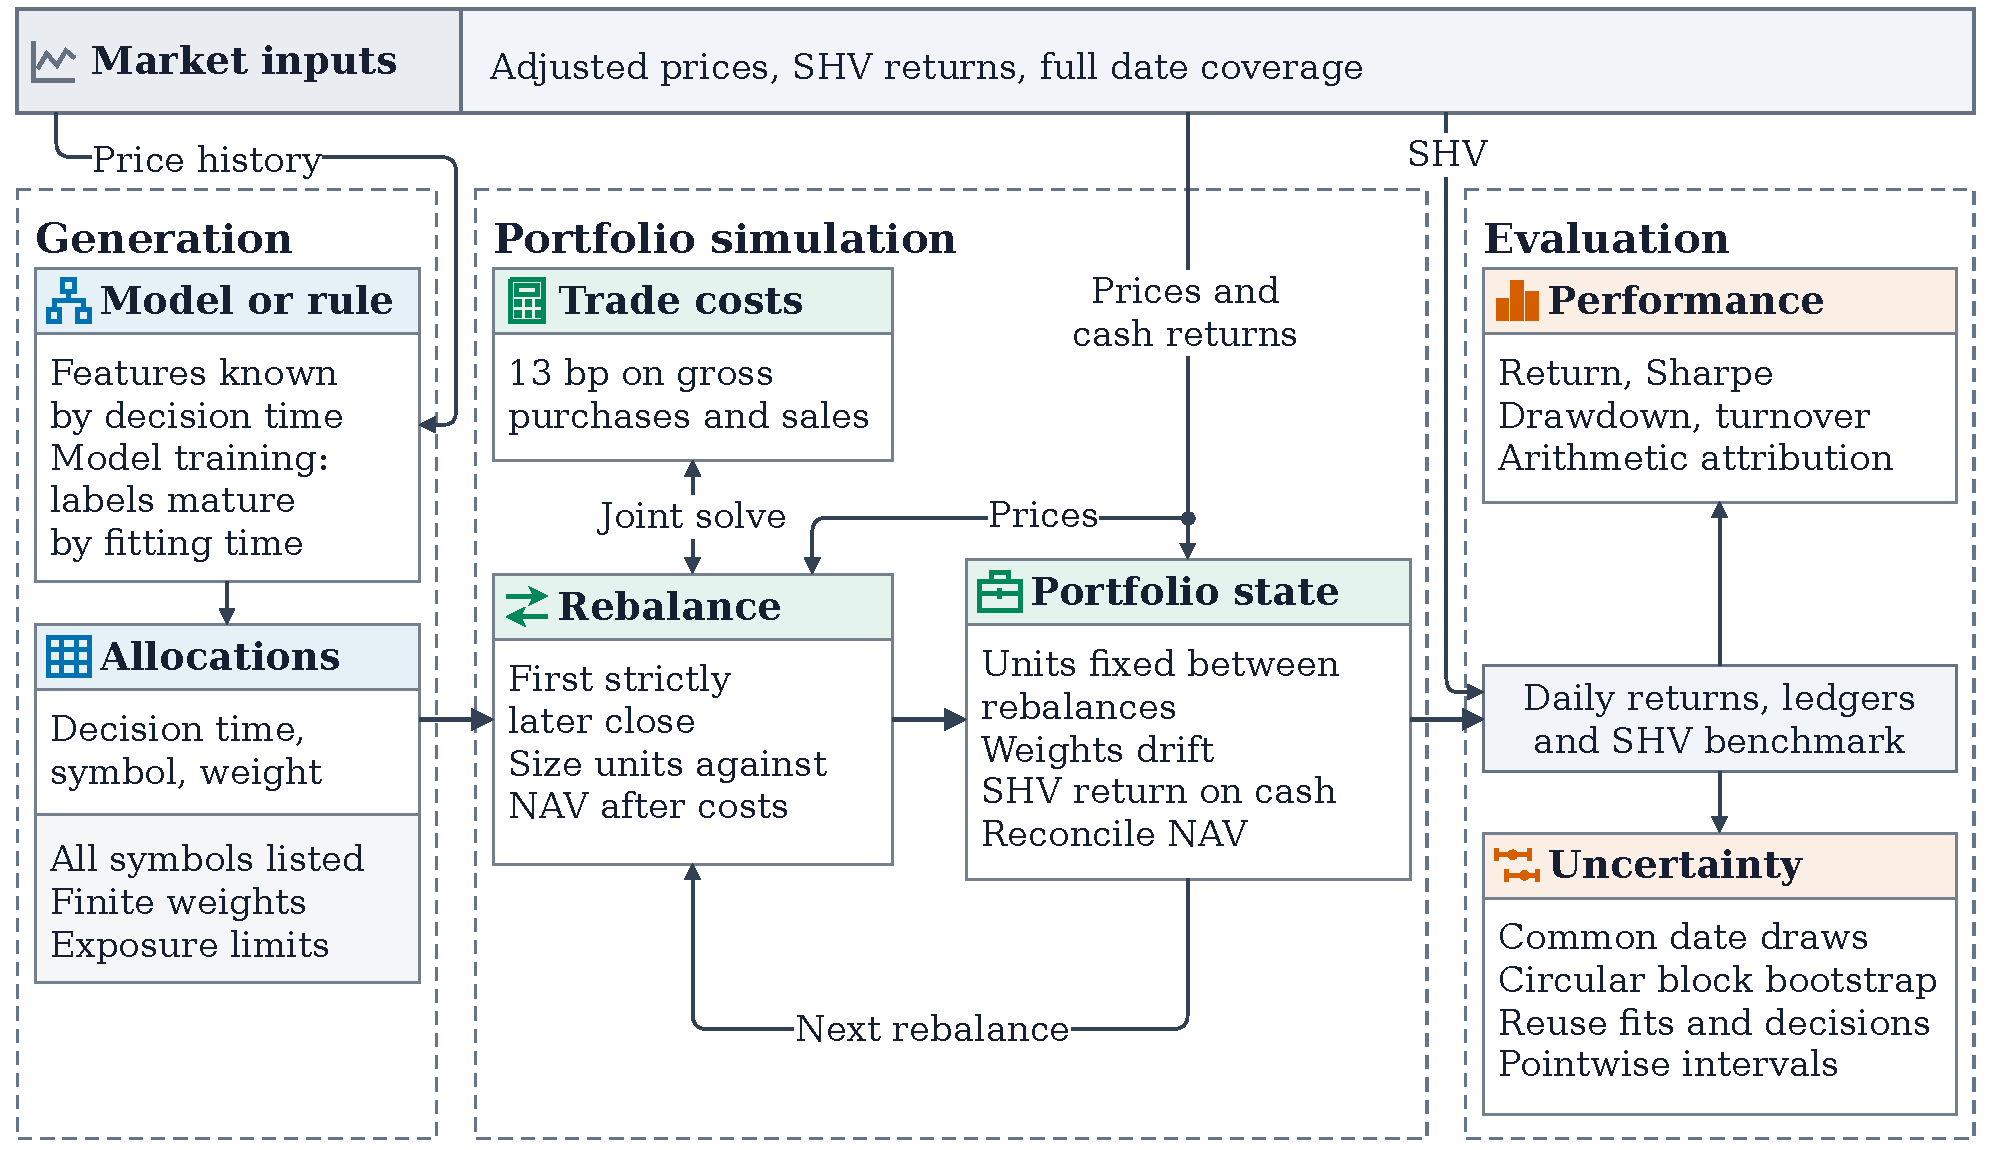
\includegraphics[width=\textwidth]{audit_protocol.pdf}
  \caption{Baseline evaluation with the event engine. Generation limits features by decision time and training labels by fitting time. The engine solves for trade quantities and costs together. Fees reduce NAV at execution; new units earn returns over the next interval. Timing, cash, and cost comparisons rerun the same targets under each convention, then align both return paths with SHV. Performance statistics and circular block resampling use these daily records. Resampling keeps the fitted models, portfolio decisions, and seeds unchanged and recomputes metrics to form pointwise intervals.}
  \label{fig:protocol}
\end{figure}

\begin{table}[t]
  \caption{Evaluation rules and the checks or records used to assess them.}
  \label{tab:invariants}
  \centering
  \begin{tabular}{>{\raggedright\arraybackslash}p{0.16\linewidth}
                  >{\raggedright\arraybackslash}p{0.40\linewidth}
                  >{\raggedright\arraybackslash}p{0.34\linewidth}}
    \toprule
    Area & Rule & Check or evidence \\
    \midrule
    Allocation record & Decision timestamp, symbol, and target weight; each decision is a complete long-only book within the gross limit. & Schema and runtime checks reject records with invalid fields, incomplete books, and invalid weights. \\
    Information and timing & Features must be available by their decision times, and training labels when fitting begins. Execution uses the first later bar. & The generator checks feature and label availability. The evaluator checks execution alignment. \\
    Cash and cost & Residual cash earns the return calculated from adjusted closing prices of the Treasury ETF SHV; 13 basis points apply to gross notional bought and sold. & Checks reject missing cash returns and absent cost models; ledgers reconcile. \\
    Comparison & Basket return at actual exposure; a separate portfolio follows target exposure and pays its own costs. & Daily return reconciliation, reproducible comparisons, and cost records. \\
    Engines & Accounting quantities stay fixed between trades in the event engine; the vectorized engine resets weights daily. & Common target weights reveal differences between the accounting conventions. \\
    Order state & Record intent before submission. Prevent a retry after an uncertain outcome and a new identifier while an intent for the same symbol remains unresolved. & Simulated failures exercise stale writes, retries, and replacement identifiers in the order ledger. \\
    \bottomrule
  \end{tabular}
\end{table}

\subsection{Portfolio accounting}

A target decided at a close earns returns only on later intervals. Let
$w_d\in\mathbb{R}^N$ be the target for risky assets decided after observing the close
at decision time $d$, and let $e(d)$ be the first available execution bar
strictly after $d$. We express holdings in accounting units valued at adjusted closing prices. At $e(d)$, the primary event engine solves for quantities $q_{i,e(d)}$ against net asset value after costs, denoted NAV, so that the resulting risky
allocation matches $w_d$. These quantities remain fixed between rebalances, while portfolio weights drift as prices and NAV change. If $P_{i,t}$
is the adjusted closing price and $V_t$ is portfolio NAV, the risky weight at
the prior close is $h_{i,t-1}=q_{i,t-1}P_{i,t-1}/V_{t-1}$. The resulting holdings first earn returns over the
interval following the execution close.
For the long-only case, $h_{i,t}\geq 0$ and $\sum_i h_{i,t}\leq 1$; residual cash
is
\begin{equation}
  h^c_t = 1-\sum_{i=1}^N h_{i,t}.
\end{equation}
For simple asset returns $r_{i,t}$ over $(t-1,t]$ and return on the cash account
$r^c_t$, portfolio return before costs is
\begin{equation}
  r^{\mathrm{gross}}_t = \sum_{i=1}^N h_{i,t-1}r_{i,t}
  + h^c_{t-1}r^c_t.
  \label{eq:gross}
\end{equation}
The engine rejects gaps in a supplied series of cash returns. For the change
in executed risky notional $\Delta a_{i,t}$, measured against NAV before trading,
define $B_t=\sum_i\max(\Delta a_{i,t},0)$ and
$S_t=\sum_i\max(-\Delta a_{i,t},0)$. One-way turnover is
$\max(B_t,S_t)$. The charge applies to purchases plus sales,
$B_t+S_t$, at a rate of 13 basis points:
$\kappa_t=0.0013(B_t+S_t)$ of NAV before trading. If $V^-_t$ is NAV before trading and
$V_{t-1}$ is NAV at the prior close, the reduction in period return is
$d_t=\kappa_t V^-_t/V_{t-1}$ and
$r^{\mathrm{net}}_t=r^{\mathrm{gross}}_t-d_t$. The engine solves for accounting quantities using
NAV after costs. We use this flat charge to study sensitivity to trading. Estimating execution cost also depends on spread, market impact, order size, liquidity, volatility, and venue information \citep{almgren2001execution}. The same proportional schedule applies to every trade in these experiments.

\begin{samepage}
We report nominal compound annual growth rate, or CAGR, maximum drawdown, annualized one-way turnover, gross
traded notional, and the sample Sharpe ratio relative to benchmark returns $r^f_t$:
\begin{equation}
  \mathrm{SR}_f = \sqrt{252}\,
  \frac{\operatorname{mean}(r_t-r^f_t)}
       {\operatorname{sd}(r_t-r^f_t)}.
  \label{eq:sharpe}
\end{equation}
\end{samepage}
The baseline sets $r^c_t=r^f_t=r^{\mathrm{SHV}}_t$. The comparison with zero cash income
sets $r^c_t=0$, while the convention comparisons retain
$r^f_t=r^{\mathrm{SHV}}_t$. The cash comparison changes the portfolio's income while using the same reporting benchmark. Equation~\ref{eq:sharpe} gives the conventional descriptive annualization. Its use for inference depends on assumptions about distributions and serial dependence \citep{lo2002statistics}. We use the circular block bootstrap \citep{politis1992circular}: each draw samples sequences of consecutive dates with replacement, and wraps from the last observation to the first when a sequence crosses the sample boundary. These sequences, or blocks, retain dependence among their observations.

We credit cash with returns calculated from SHV closing prices after the provider's adjustments. SHV is a Treasury ETF, so this convention includes fund expenses, duration exposure, and changes in its market price. Risky holdings use adjusted prices as well. The resulting units serve total return accounting; implementing these positions as share purchases would also need market and execution records.

\subsection{Return decomposition}

We decompose net return in excess of cash into allocation, timing, passive exposure, and cost. Let $x_t=\sum_i h_{i,t-1}$ be risky exposure during return period $t$,
let $b_t$ be the return of a buy-and-hold basket with equal initial weights, and let
$\bar{x}$ be the mean of $x_t$ over the full sample. Basket returns at actual exposure and at mean exposure are
\begin{align}
  m_t &= x_t b_t + (1-x_t)r^c_t, \\
  k_t &= \bar{x} b_t + (1-\bar{x})r^c_t.
\end{align}
Then net excess over cash has the exact arithmetic decomposition
\begin{align}
  r^{\mathrm{net}}_t-r^c_t
  ={}& \underbrace{(r^{\mathrm{gross}}_t-m_t)}_{\text{active risky allocation}}
  + \underbrace{(m_t-k_t)}_{\text{dynamic exposure timing}} \nonumber\\
  &+ \underbrace{(k_t-r^c_t)}_{\text{passive risky exposure}}
  + \underbrace{(r^{\mathrm{net}}_t-r^{\mathrm{gross}}_t)}_{\text{implementation cost}}.
  \label{eq:decomposition}
\end{align}
The allocation term combines group selection, weights within the risky portfolio, and drift between rebalances. Its reference is the basket return at the strategy's actual exposure. Brinson selection instead weights return differences within groups by benchmark group weights. These definitions answer different attribution questions.

The timing term compares exposure on each day with its mean over the evaluation window. It is positive when exposure is above that mean and the basket outperforms cash, or when exposure is below the mean and the basket underperforms cash. The mean uses the full sample, so the timing term describes the return history ex post. Interpreting the terms as causal effects or as returns on separately tradable portfolios involves assumptions beyond this accounting decomposition.

Averaging the daily components and multiplying by 252 gives their annualized arithmetic contributions. These contributions add to annualized mean return above cash. CAGR instead compounds the daily net returns, so it has a different aggregation rule.

We resample the five series in Equation~\ref{eq:decomposition} together, using the same sequences of consecutive dates. Their component means add to mean net return above cash in every resample. Each component's interval uses its own percentiles of the resampling distribution. Adding these component bounds generally gives different endpoints from the interval for mean net return above cash. The fraction of positive resamples describes the distribution of the estimated mean.

\subsection{Accounting comparisons}

Three comparisons reuse the same portfolio decisions, input prices, and primary engine. Each changes one convention: cash earns zero, the proportional trading charge is removed, or a new allocation receives the return interval ending at its decision close. The last convention assigns a past return to a decision made after observing that close. It is deliberately infeasible and tests the effect of incorrect return timing.

Cash income and trading charges change NAV, which can affect subsequent exposure and trade size even when the target weights stay the same. Our reruns include those accounting consequences. Following \citet{zhang2026alpha}, each of these comparisons changes one convention. The basket and engine comparisons described below change several aspects of the calculation together.

\subsection{Validation checks}

The checks cover allocation sums, position limits, exposure after overlays, and information availability. Each evaluation starts from a complete allocation record. In both studies, the strategy's decisions also determine the comparison portfolio's exposure, letting us examine how different allocations and accounting rules turn those decisions into returns.

Synthetic examples with answers calculated by hand check the accounting independently of market data. The experiment records identify the inputs, settings, and software environment needed to repeat each calculation. Separate order tests simulate stale state, an uncertain submission outcome, and a replacement order for the same symbol. The submission record must retain the earlier intent and prevent a second submission until the outcome is reconciled. Appendix~\ref{app:evidence} distinguishes this test evidence from the checks needed for live execution.

\section{Evaluation design}

\subsection{Retrospective audit}

The first study evaluates a weekly rotation strategy on six ETFs from
January 2, 2018, through December 31, 2025. It combines group ranking, residual momentum, exposure states from a Gaussian mixture, and volatility scaling. The strategy predates the audit, and the number of earlier trials is unknown. We retain that history as the object of the accounting investigation.

The original strategy contains a defect that matters for interpreting its returns. QQQ is both a group member and the ranking benchmark. Its regression on itself should give zero residuals, but positive rounding error can survive the score filter and receive substantial weight after normalization. Two regime features are exact rescalings of the same volatility series, early regime windows contain little fitting history, and one seed determines the mixture fit. We preserve these choices, including the QQQ defect, to audit the strategy's original portfolio decisions. Appendix~\ref{app:retrospective} gives the rule.

The event engine credits cash with SHV returns, charges 13 basis points on purchases and sales, and executes each weekly allocation at the first later close. The decomposition uses the return of a basket at the strategy's actual exposure before costs. A separate comparison portfolio starts with equal basket weights, lets their composition drift, follows the strategy's target exposure, and pays its own trading charges. Both portfolios use the same execution timing and cash convention. This comparison measures the contribution of allocation choices after costs along the strategy's exposure schedule.

\subsection{Expansion study}

We wrote the second study's protocol before requesting its data. Because the evaluation period had already occurred, this chronology limits discretion over the analysis of a historical sample. It does not create an independent test period. Section~\ref{sec:limitations} discusses historical reuse and the absence of external registration.

Two ETF sets use adjusted closing prices from January 2, 2014, through
December 31, 2025. The sector set contains XLB, XLE, XLF, XLI, XLK, XLP, XLU, XLV, and
XLY. The country set contains EWA, EWC, EWG, EWH, EWJ, EWL, EWP, EWQ, EWS, and
EWU. Each also includes SHV. Evaluation covers \ExpansionEvaluationSessions{}
sessions from January 2, 2018, through December 31, 2025. Each dataset keeps only sessions with observations for every required symbol. Preprocessing excludes forward filling and symbol substitution. The sets consist of surviving funds with shared market exposures, so their results describe related parts of the same history.

Table~\ref{tab:expansion-design} gives the target rules. Each monthly decision
uses the first complete session and executes on the first strictly later close.
The fraction allocated to risky assets is at most one, with short positions excluded; idle capital earns SHV returns. The event
engine holds quantities valued at adjusted closing prices fixed between rebalances and charges 13
basis points for every dollar bought or sold, using the $B_t+S_t$ cost base defined above. The evaluator checks the target weights before calculating returns. The comparator
preserves target gross risky exposure, divides it equally across the risky ETFs, excluding SHV, at
each decision, then executes at the first later close, credits residual cash with SHV returns, and pays its
own trading charges.

\begin{table}[t]
  \caption{Portfolio rules in the expansion study. Gradient boosting fits regression trees, abbreviated GBRT in the plots. Ties use ascending symbols. Reversal and gradient boosting assign one-third to each qualifying asset, leaving the unused allocation in cash when fewer than three qualify.}
  \label{tab:expansion-design}
  \centering
  \begin{tabular}{>{\raggedright\arraybackslash}p{0.22\linewidth}
                  >{\raggedright\arraybackslash}p{0.70\linewidth}}
    \toprule
    Family & Portfolio rule \\
    \midrule
    Time series momentum & Positive simple returns over 252 sessions; equal weight on qualifying assets; hold cash if none qualify. \\
    Cross-sectional momentum & Three highest simple returns from $t-252$ to $t-21$; one-third each. \\
    Short-term reversal & Up to three lowest negative simple returns over 5 sessions; one-third each, without renormalizing. \\
    Gradient boosting & Up to three highest strictly positive predictions of log return over 21 sessions; one-third each, without renormalizing; five seeds. \\
    \bottomrule
  \end{tabular}
\end{table}

At each monthly decision, we fit one regressor per seed to observations pooled across the risky assets in that ETF set. A training row is eligible once its return outcome can be observed at that close. Features use prices available by their own decision dates. Appendix~\ref{app:expansion-targets} gives the feature windows, return label, training window, model settings, and seeds.

Each seed produces its own allocation record and portfolio returns. We calculate metrics separately for those portfolios, then average the five values. The gradient boosting Sharpe entry is the average of the five individual ratios. A portfolio that combines their holdings would be a different investment strategy.

\subsection{Comparison design}

Five comparisons use the same dates and the subtraction directions below. Three change one accounting convention while reusing the allocation records:
retroactive close assignment minus execution at the first later close, zero return on residual cash minus SHV cash, and zero trading charge minus the charge of 13 basis points.
The fourth subtracts the performance of the comparison portfolio after its own costs from that of the net strategy, with both executing at the first later close and using the same target exposure.
The fifth subtracts performance under event engine accounting from performance under vectorized accounting. The comparator changes
cross-sectional allocation, turnover, and cost. The engine comparison combines
daily weight resets, weight drift, trade accounting, and sizing after costs. Each comparison uses a separate rerun. Runs combining the changes would measure their joint effect.
If the target on the first evaluation date is nonzero, retroactive assignment charges its initial entry before the evaluation window; execution at the first later close charges it inside the window. The timing contrast also includes that difference in the timing of entry costs.

Primary outcomes are differences in annualized arithmetic return and
sample Sharpe relative to SHV. We construct unstudentized pointwise 95\%
percentile intervals from \ExpansionBootstrapReplications{} circular block resamples
of aligned daily observations. The primary block contains 21 consecutive sessions; sensitivity checks use 5 and 63 sessions
\citep{politis1992circular}. Within each family and ETF set, both sides of a comparison and SHV use the same sampled dates. For gradient boosting, those dates are shared by all five seed pairs. Model fits, ETF sets, families, allocation records, design choices, and seeds are held unchanged during resampling. Each interval describes one comparison under those conditions. Section~\ref{sec:limitations} addresses multiplicity and the uncertainty that this resampling leaves outside its scope.

\section{Results}

\subsection{Performance across ETF sets}

Sector ETFs outperform country ETFs on arithmetic return, compound growth, and Sharpe relative to SHV for all four strategy families over this period. Country time series momentum illustrates why the cash benchmark matters: its nominal return is positive, but its return relative to SHV gives a slightly negative Sharpe ratio. Capital growth alone misses that opportunity cost.

The risk comparison between gradient boosting and cross-sectional momentum reverses across ETF sets. For country ETFs, the regression portfolios have lower mean compound growth, and every seed has lower volatility and a shallower drawdown than the momentum rule. For sector ETFs, every seed has higher volatility and a deeper drawdown. The model's risk profile depends on the investment universe even with the same fitting procedure. Appendix Table~\ref{tab:expansion-baseline} reports the eight cases, and Figure~\ref{fig:expansion-baseline} compares return and Sharpe estimates. Model entries average metrics from separate seed portfolios.

\subsection{Effects of accounting conventions}

Retroactive close assignment has its largest effect on arithmetic return for short-term reversal. The rule selects assets with negative recent returns using a window that includes the decision close. Assigning those assets to the interval ending at that close credits the portfolio with a return that helped select them. The observed direction is consistent with that mechanism: annualized arithmetic return falls by about seven percentage points in each ETF set. Both pointwise intervals from blocks of 21 sessions lie below zero. Sector gradient boosting is the third case with an interval below zero among the eight timing comparisons in Appendix Figure~\ref{fig:contract-return}.

Time series momentum moves in the opposite direction: retroactive assignment raises its return in both sets, although both pointwise intervals include zero. Together, the opposite signs show how a timing error can produce an apparently conservative result. Feasibility depends on the order of observation, decision, execution, and return, regardless of which direction the performance statistic moves. Appendix~\ref{app:timing-example} illustrates both signs with two assets.

Cash effects depend on how much capital remains uninvested and when. Cross-sectional momentum stays almost fully invested and changes little when cash earns zero. Reversal holds more cash, especially in countries, and loses more income under that convention. Five of the eight pointwise cash intervals lie below zero. SHV remains the reporting benchmark in both runs, so the comparison captures cash income and its subsequent effects on NAV and holdings.

Removing trading charges raises annualized arithmetic return by \ExpansionCostEffectRange{}, with all eight pointwise intervals above zero. Differences in the amount traded explain much of the variation in cost effects across strategies. Country reversal trades substantially more gross notional per year than sector time series momentum, and multiplying traded notional by the charge approximates the corresponding return reduction. The full comparison measures sensitivity to this proportional cost assumption by rerunning the portfolios, since charges also change NAV and later trade sizes.



\subsection{Strategy rankings}

Accounting conventions also change the sample ranking of the strategies in Table~\ref{tab:rank-sensitivity}. Retroactive assignment swaps gradient boosting with time series momentum in sectors, and reversal with time series momentum in countries. Removing trading costs swaps reversal with time series momentum in sectors and puts gradient boosting above cross-sectional momentum in countries. Each alternative produces one pairwise swap in each ETF set.

Some ranking changes reflect small Sharpe differences. With zero cost, sector reversal and time series momentum differ by about 0.006, which disappears when both ratios are rounded to two decimal places. We retain three decimals in the table for that reason. These sample rankings describe the observed portfolios. Appendix Figure~\ref{fig:contract-sharpe} instead gives pointwise intervals for the change in each strategy's Sharpe when its accounting convention changes.

\begin{table}[t]
  \centering
  \caption{Sample Sharpe relative to SHV and rank within each ETF set. Rank one is highest. Bold marks the highest sample Sharpe within each set and convention. Each alternative changes timing or trading cost separately from the baseline. Retroactive assignment is infeasible and can move the initial entry charge outside the evaluation window. Zero trading cost retains baseline timing and cash income. Gradient boosting entries average five individual seed Sharpes.}
  \label{tab:rank-sensitivity}
  \setlength{\tabcolsep}{5pt}
  \begin{tabular}{@{}lrrrrrr@{}}
    \toprule
    & \multicolumn{2}{c}{Baseline}
    & \multicolumn{2}{c}{Retroactive assignment}
    & \multicolumn{2}{c}{Zero trading cost} \\
    & & & \multicolumn{2}{c}{\textit{infeasible}} & & \\
    \cmidrule(lr){2-3}\cmidrule(lr){4-5}\cmidrule(l){6-7}
    Strategy & \shortstack{Sharpe\\ratio} & Rank & \shortstack{Sharpe\\ratio} & Rank & \shortstack{Sharpe\\ratio} & Rank \\
    \midrule
    \ExpansionRankRows
    \bottomrule
  \end{tabular}
\end{table}

\subsection{Sources of return}

The comparison portfolios follow each strategy's target exposure, execution timing, and cash convention, but replace its risky allocation with a basket that pays its own trading costs. The retrospective basket starts with equal weights and then drifts; the expansion basket returns to equal weights at every decision. These comparisons ask whether the allocation rule improves performance along the same intended exposure schedule after trading costs. Seven of the eight expansion intervals for annualized arithmetic return include zero. Country time series momentum is the exception, with a negative difference from its basket and a pointwise interval below zero. Positive nominal returns can coexist with little evidence of an allocation advantage.

Cash treatment is especially consequential for the retrospective strategy. It spends \PaperFullyCash{} of the sample entirely in cash. Its compound growth falls below SHV despite that cash income and falls further when cash earns zero. The arithmetic decomposition shows a corresponding shortfall in mean return above cash: active allocation and trading costs outweigh positive contributions from passive exposure and exposure timing.

The pointwise interval for the allocation contribution lies below zero. Appendix Table~\ref{tab:decomposition} reports all component estimates and intervals; their means add to net return above cash before rounding. This accounting decomposition identifies where the observed shortfall arises under the chosen basket reference.

The comparison with a basket after its own costs answers a different question. The decomposition holds the strategy's actual exposure when attributing allocation return; the comparison portfolio follows target exposure and incurs its own trades and charges. Differences in exposure and cost treatment explain why its return comparison differs from the allocation component. Appendix~\ref{app:retrospective-results} reports both calculations.

\subsection{Sensitivity checks}

Appendix Figure~\ref{fig:seed-sensitivity} compares the regression portfolios for the five seeds with the simple trading rules. The mean Sharpe summarizes the five portfolios under one training design. Evaluating a portfolio that combines their holdings would require calculating its own return series and Sharpe ratio.

The mean can conceal differences in model ranking. In sectors, four of the five regression runs exceed time series momentum on Sharpe relative to SHV, but only one exceeds cross-sectional momentum. In countries, every run exceeds time series momentum and two exceed cross-sectional momentum. Those two also have higher CAGR than cross-sectional momentum, even though every regression run has lower annualized arithmetic mean return. Sharpe uses both the mean and standard deviation of returns above cash; CAGR compounds daily returns. Model comparisons depend on the metric and seed within this shared historical sample. Appendix~\ref{app:expansion-followups} examines convention effects, annual excess returns, and trading for each seed.

The engine comparison changes how portfolio decisions become daily holdings. Both engines receive the same target weights and prices. The vectorized calculation resets weights to the last executed vector each day; the event engine keeps quantities unchanged between trades, so weights move with prices. The engines also differ in trade accounting and sizing after costs. Appendix Figure~\ref{fig:engine-sensitivity} reports the largest absolute daily return difference for each family and ETF set.

The largest absolute daily return difference occurs for sector gradient boosting, while sector cross-sectional momentum has the largest difference in final wealth, \ExpansionEngineMaxWealthGap{} of initial capital. We calculate final wealth by compounding each engine's return series separately. The largest daily difference and the final wealth difference measure different aspects of engine behavior, since daily differences can accumulate or offset one another.

The retrospective strategy's returns agree much more closely across the engines. Engine sensitivity depends on both the portfolio decisions and the accounting conventions.

Changing the resampling block length leaves the interval conclusions for timing, cost, and the basket comparisons unchanged across 5, 21, and 63 sessions, as summarized in Appendix Table~\ref{tab:effect-counts}. The small sector gradient boosting cash effect includes zero with the longest blocks. For engine differences, the treatment of temporal dependence changes the interval conclusions: two intervals for annualized arithmetic return lie above zero with blocks of 5 sessions, compared with four for blocks of 21 and 63 sessions.

\subsection{Performance across subperiods}

The retrospective strategy has higher CAGR but lower Sharpe relative to SHV in 2022 through 2025 than in 2018 through 2021. The comparison basket exceeds the strategy on both measures in each half, so its advantage over the full sample also appears in both subperiods. These comparisons divide the original return history without changing its portfolio decisions.

\section{Limitations}
\label{sec:limitations}

Both studies use historical periods available during development. Earlier trials of the rotation strategy are incompletely recorded, and the expansion protocol remains under author control without external registration. The comparisons establish accounting effects for these strategies on these histories. Assessing performance on an independent sample means setting aside a period throughout development or collecting future observations.

The ETF sets share dates and market exposures, and the five seeds repeat one model specification. Pointwise intervals describe resampling of daily returns conditional on the models and portfolio decisions already used. Nominal coverage relies on stationarity, sufficiently weak dependence, and suitable moment conditions. These intervals exclude uncertainty from model selection and from sampling a wider population of seeds. Simultaneous coverage requires a multiplicity procedure. The incomplete search history also prevents calculation of a Deflated Sharpe Ratio or a White Reality Check \citep{white2000reality,bailey2014deflated}. Appendix~\ref{app:scope} explains these limits and the dependence assumptions.

Historical accounting and live execution provide different kinds of evidence. Capacity and execution quality depend on liquidity, order size, market impact, and venue conditions beyond the flat charge used here. Simulated order tests check particular failure scenarios; broker behavior during live operation needs separate observation. Treating these conditional comparisons as evidence for live deployment could expose investors to losses from underestimated risk or trading costs. This audit helps a reader inspect the assumptions behind a performance claim before using it to inform an investment decision.

\section{Conclusion}

A model's portfolio decisions acquire a performance history through execution and accounting rules. Our comparisons show that an infeasible timing convention can raise or lower measured performance, while cash income and trading intensity also affect it. The retrospective decomposition traces the shortfall relative to cash to allocation and costs despite positive exposure and timing contributions. Interpreting model performance requires this connection between the information available at the decision, the holdings that follow execution, and the cash flows that produce the return.

\clearpage
\ifquantcortexreview
\begin{ack}
We thank the yfinance contributors for maintaining the software used to retrieve Yahoo Finance price data, and the NumPy, pandas, scikit-learn, and Matplotlib contributors for the analysis and plotting tools. The work had no external funding, and we have no competing interests to disclose.
\end{ack}
\fi

\FloatBarrier
\bibliographystyle{plainnat}
\bibliography{references}
\ifquantcortexreview\else
  \clearpage
\fi

\appendix
\raggedbottom

\section{Scope of the evidence}
\label{app:scope}

Adjusting inference for strategy search requires a record of the trials. The Deflated Sharpe Ratio uses the effective number of independent trials and the variance across trial Sharpe estimates, together with the selected return series' Sharpe ratio, length, skewness, and kurtosis. White's Reality Check requires a candidate universe, benchmark, performance criterion, and observations suitable for joint resampling or equivalent retained summaries \citep{white2000reality,bailey2014deflated}. The available trial history is incomplete, so we report sample metrics and conditional intervals.

The allocation component can also be written as
$A_t=\sum_i h_{i,t-1}(r_{i,t}-b_t)$, a contribution per unit of portfolio capital.
This expression remains defined when the portfolio holds only cash.
For the timing component, let $T_t=m_t-k_t$, $z_t=b_t-r_t^c$, and let
$\bar{z}$ denote the mean over the $n$ evaluation sessions. Then
\begin{equation}
  252\bar{T}
  = \frac{252}{n}\sum_{t=1}^{n}(x_t-\bar{x})(z_t-\bar{z}).
  \label{eq:timing-covariance}
\end{equation}
The mean timing contribution is positive when exposure and basket excess return
move together over the sample. Its annualized mean equals 252 times their
empirical covariance, calculated with denominator $n$. The basket at mean
exposure uses an ex post reference; a causal timing interpretation or a
separately tradable timing strategy requires additional assumptions. The
bootstrap resamples the precomputed components while keeping the original
$\bar{x}$ fixed, so every draw uses the same reference.

The decomposition describes arithmetic excess return; geometric linking needs a separate construction. The fraction of bootstrap draws with a positive mean is a frequency within the resampling distribution. Posterior probabilities need a Bayesian probability model, and inference across multiple comparisons needs an appropriate testing procedure.

The datasets contain funds available at the time of collection. Point-in-time constituent histories would change the investment opportunity set. Country ETFs are unhedged securities listed in the U.S., so currency and overlapping market exposures enter their returns. SHV contributes duration, expenses, and variation in market prices to the cash proxy. The quantities valued at adjusted closing prices are units for total return accounting. Executable share quantities, spreads, market impact, volume constraints, and fill uncertainty would require additional market and broker records.

The regression model uses one specification and five fixed seeds. It pools asset observations within each ETF set without using the symbol as a feature. The bootstrap conditions on the resulting fitted models and target weights. Nominal coverage relies on stationarity, sufficiently weak dependence, suitable moment conditions, and an appropriate block construction. We compare three block lengths to assess interval sensitivity. This comparison does not test the assumptions on the return process. The uncertainty estimates exclude model selection, hyperparameter search, population variation across seeds, and future performance.

The audit tests particular invariants and failure cases. Estimating a rate of defect detection would need a defined population of faulty implementations, and measuring the incremental value of a check would need comparisons with procedures that omit it. The convention and overlay comparisons measure changes in portfolio accounting and exposure.

The simulated order tests exercise stale state, uncertain retries, and replacement identifiers. The order ledger stops a new order while an earlier intent for the same symbol remains unresolved, so even a valid later order may wait for reconciliation. Establishing pending exposure across the account, delivery semantics across concurrent clients, authenticated transport, and venue behavior requires further operational evidence. These are prerequisites for assessing a funded deployment.

\subsection{A worked example of retroactive assignment}
\label{app:timing-example}

Consider two assets observed at four successive closes, with prices given below. Starting wealth is $1$, held entirely in cash, and both cash return and trading charge are zero. After observing $t_1$, a winner rule selects A, while a loser rule selects B; either rule targets full investment in the selected asset. These rules illustrate one interval. The empirical time series momentum and reversal rules use 252 and 5 sessions, respectively.

\begin{center}
  \begin{tabular}{@{}lrrl@{}}
    \toprule
    Close & Price of A & Price of B & Feasible chronology \\
    \midrule
    $t_0$ & 100 & 100 & Entirely in cash \\
    $t_1$ & 110 & 90 & Observe prices and select A or B \\
    $t_2$ & 110 & 90 & Execute the selected target \\
    $t_3$ & 110 & 90 & First return earned by the new holding \\
    \bottomrule
  \end{tabular}
\end{center}

Feasible execution occurs at $t_2$. The new holding first earns the return ending at $t_3$, which is $110/110-1=0$ for A and $90/90-1=0$ for B. Both feasible portfolios therefore finish with wealth $1.00$.

Retroactive assignment instead credits the already ended interval from $t_0$ to $t_1$: $110/100-1=+0.10$ for A or $90/100-1=-0.10$ for B. Subsequent prices are unchanged, so the fictitious terminal wealth is $1.10$ or $0.90$.

The same chronology error creates a gain for the winner rule and a loss for the loser rule. This example isolates return timing. The empirical comparison uses a trading charge of 13 basis points and includes any shift of the initial entry charge across the evaluation boundary.

\section{Retrospective case specification}
\label{app:retrospective}

The universe is QQQ, VGT, GLD, TLT, SPY, and VIG, grouped as growth equities,
gold and nominal duration, and broad and dividend equities. On the first session
of each week, the strategy keeps the top two groups by an information
ratio over 126 sessions relative to QQQ. Within selected groups, it estimates a regression on one factor over 126 sessions,
then sums residual returns over the next 126 sessions, leaving the most recent
21 sessions out of score formation. Each residual equals the asset return minus the fitted intercept
and benchmark contribution, and enters the score in return units with coefficient one.
Positive scores receive proportional long-only
weights capped at 60\% per asset.

A Gaussian mixture with three components and full covariance uses seed 42, covariance
regularization $10^{-5}$, and at most 100 iterations. It maps QQQ return and two
exact rescalings of realized volatility over 20 sessions to zero, half, or full
exposure. A separate volatility scaler uses 21 sessions, targets 20 volatility points,
and clips its multiplier to $[0.3,1.0]$. The strategy requires 274 sessions of history before evaluation; 503 are available. If a benchmark, group signal, or regression estimate
is unavailable, it falls back to plain momentum. It holds cash if all mature
residual scores in the selected groups are nonpositive. The comparison evaluates all named variants: removing the regime rule, removing the volatility scaler, and removing both.

\clearpage
\subsection{Retrospective accounting results}
\label{app:retrospective-results}

\begin{table}[h]
  \caption{Retrospective performance under baseline accounting from 2018
  through 2025. Every Sharpe in the table uses SHV as its reporting benchmark. The
  path with zero return on residual cash retains SHV as the reporting benchmark. Its Sharpe against zero is \PaperZeroCashSharpe{}. The comparison portfolio executes at the first later close and matches the strategy's target exposure.}
  \centering
  \setlength{\tabcolsep}{4pt}
  \begin{tabular}{@{}lrrr@{}}
    \toprule
    Series & \shortstack{Compound\\annual\\growth rate} & \shortstack{Sharpe\\ratio} & \shortstack{Maximum\\drawdown} \\
    \midrule
    Strategy, after costs, with SHV cash & \PaperNetCAGR & \PaperNetSharpe & \PaperNetMaxDrawdown \\
    Strategy, before costs, with SHV cash & \PaperGrossCAGR & \PaperGrossSharpe & \PaperGrossMaxDrawdown \\
    SHV cash proxy & \PaperCashCAGR & Undefined & \PaperCashMaxDrawdown \\
    Basket at actual exposure, before costs & \PaperMatchedCAGR & \PaperMatchedSharpe & \PaperMatchedMaxDrawdown \\
    Comparison portfolio, after costs & \PaperCostedComparatorCAGR & \PaperCostedComparatorSharpe & \PaperCostedComparatorMaxDrawdown \\
    Strategy, after costs, with zero cash return & \PaperZeroCashCAGR & \PaperZeroCashSHVSharpe & \PaperZeroCashMaxDrawdown \\
    \bottomrule
  \end{tabular}
\end{table}

After each portfolio pays its own trading costs, the annualized arithmetic mean of daily strategy returns minus comparison returns is \PaperCostedActiveMean{}. Resampling those differences in circular blocks of 21 sessions gives a pointwise 95\% percentile interval from \PaperCostedActiveLower{} to \PaperCostedActiveUpper{}, conditional on the observed portfolio decisions.

\begin{table}[h]
  \caption{Exact attribution of annualized arithmetic net
  excess return over SHV. Pointwise intervals use common resamples of blocks of 21 sessions.
  The daily decomposition holds in each draw, and component means sum to net excess
  before rounding. Values are rounded to two decimals.}
  \label{tab:decomposition}
  \centering
  \begin{tabular}{lrrr}
    \toprule
    Component & Mean & 95\% interval & \shortstack{Draws with a\\positive mean} \\
    \midrule
    \PaperDecompositionRows
    \bottomrule
  \end{tabular}
\end{table}

\begin{center}
  \centering
  \leavevmode\vbox{\refstepcounter{figure}%
  \hbox{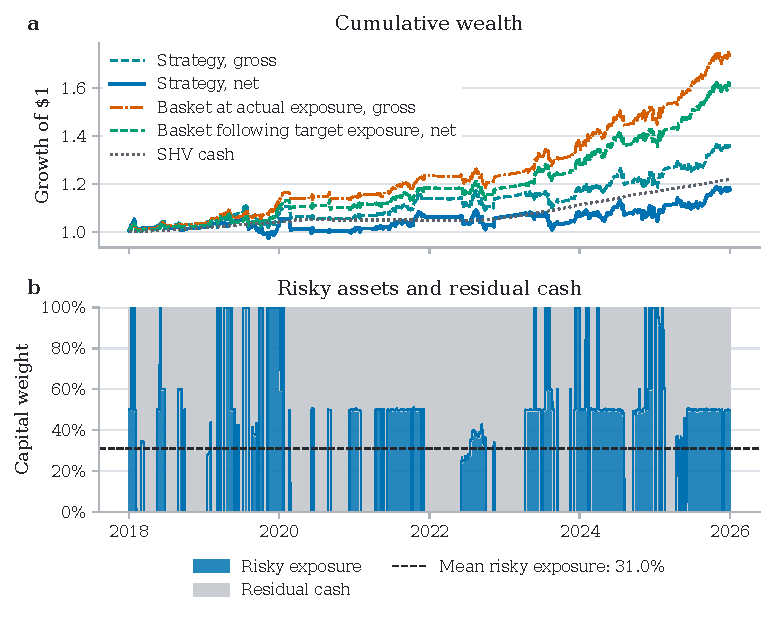
\includegraphics[width=0.92\textwidth]{accounting_summary.pdf}}}
  \parbox{0.92\textwidth}{\small Figure~\thefigure: Growth of one dollar and allocation to risky assets and residual cash in the retrospective study. Exposure is indexed by the ending date of each return interval. Cash earns SHV returns. Residual cash accounts for most capital on average.}
\end{center}

\begin{center}
  \centering
  \leavevmode\vbox{\refstepcounter{figure}%
  \hbox{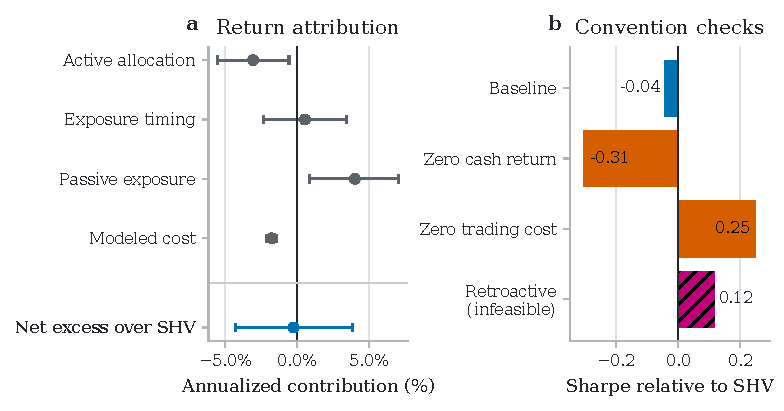
\includegraphics[width=0.92\textwidth]{return_attribution_and_protocol_switches.pdf}}}
  \parbox{0.92\textwidth}{\small Figure~\thefigure: Retrospective attribution and convention checks. Subplot a reports annualized arithmetic contributions to excess return over SHV, with pointwise 95\% intervals from common draws using circular blocks of 21 sessions. The separate bottom row sums the four component means and has its own interval from the common draws. Subplot b gives Sharpe levels relative to SHV under each convention. Hatching marks retroactive assignment, which credits a target with an interval that has already ended.}
\end{center}

\section{Code and data availability}
\label{app:reproducibility}

The public materials include the code, aggregate results, software environment specification, and synthetic accounting examples. The historical price matrices and empirical target weights are not distributed. Reproducing the reported returns requires access to the original inputs and the stated software environment. Prices were retrieved from Yahoo Finance through yfinance; later downloads may reflect revisions to historical prices. Permission from the data provider to publish derived aggregates or redistribute source data remains unverified. The synthetic examples allow the accounting checks to run without market data.

\section{Expansion results}

\refstepcounter{table}
\label{tab:expansion-baseline}
\begin{center}
  \parbox{\textwidth}{\small Table~\thetable: Expansion performance after the proportional trading charge, with Sharpe ratios relative to SHV. Bold marks the highest arithmetic return, Sharpe ratio, and compound growth and the shallowest drawdown within each ETF set, using unrounded values. These are sample rankings; uncertainty in differences requires a separate comparison. For gradient boosting, each metric is calculated separately for all five seeds and then averaged. This order also applies to compound annual growth and maximum drawdown.}
  \smallskip
  \setlength{\tabcolsep}{3.5pt}
  \begin{tabular}{@{}llrrrr@{}}
    \toprule
    Fund set & Strategy & \shortstack{Annualized\\arithmetic\\return} & \shortstack{Sharpe\\ratio} & \shortstack{Compound\\annual\\growth rate} & \shortstack{Maximum\\drawdown} \\
    \midrule
    \ExpansionBaselineRows
    \bottomrule
  \end{tabular}
\end{center}

\refstepcounter{table}
\label{tab:effect-counts}
\begin{center}
  \parbox{\textwidth}{\small Table~\thetable: Sensitivity to resampling block length. Each cell counts pointwise intervals below zero, including zero, and above zero, in that order, across eight dependent strategy and ETF set cases. Return differences are annualized arithmetic means; Sharpe differences use SHV as the benchmark. We vary the number of consecutive sessions per block while keeping the fitted models and portfolio decisions fixed. Simultaneous inference across cases requires a multiplicity adjustment.}
  \smallskip
  \begin{tabular}{@{}lccc@{}}
    \toprule
    Metric & 5 sessions & 21 sessions & 63 sessions \\
    \midrule
    \ExpansionEffectRows
    \bottomrule
  \end{tabular}
\end{center}

Return and Sharpe can indicate different directions of change in the same comparison. With the primary blocks of 21 sessions in Figures~\ref{fig:contract-return} and~\ref{fig:contract-sharpe}, all 40 pairs of intervals occupy the same position relative to zero, and 39 pairs of point estimates share a sign. The exception is the sector regression model against its comparison portfolios after trading costs: its mean annualized arithmetic return is higher by 1.04 percentage points, but its mean Sharpe is lower by 0.023. Both intervals include zero.

For two return paths on the same dates, let $\mu_j=252\,\operatorname{mean}(r_j-r^{\mathrm{SHV}})$
and $\sigma_j=\sqrt{252}\,\operatorname{sd}(r_j-r^{\mathrm{SHV}})>0$
for $j\in\{A,B\}$, using the sample standard deviation. Then
\begin{equation}
  \mathrm{SR}_A-\mathrm{SR}_B
  = \frac{\mu_A-\mu_B}{\sigma_A}
  + \mu_B\left(\frac{1}{\sigma_A}-\frac{1}{\sigma_B}\right).
  \label{eq:paired-sharpe}
\end{equation}
The common SHV series makes $\mu_A-\mu_B$ equal to the difference in annualized
arithmetic returns. Equal standard deviations of returns above SHV preserve its sign;
different standard deviations can change the ordering. For the regression model,
the equality holds for each seed pair before averaging.

\begin{center}
  \centering
  \leavevmode\vbox{\refstepcounter{figure}%
  \label{fig:expansion-baseline}%
  \hbox{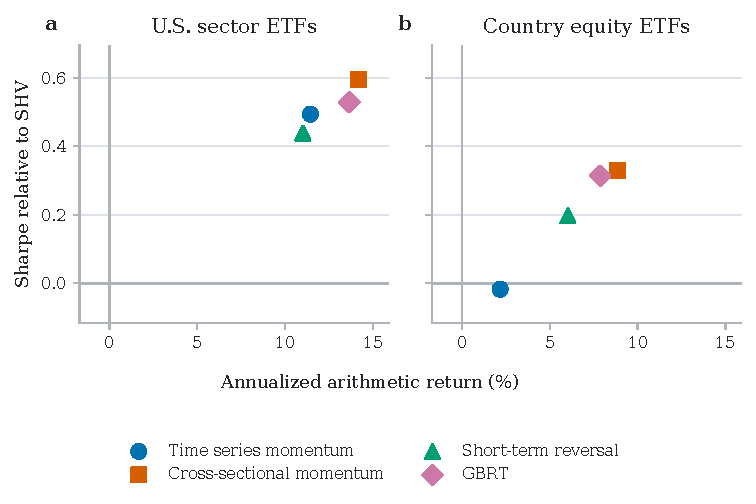
\includegraphics[width=0.90\textwidth]{baseline_performance.pdf}}}
  \parbox{0.90\textwidth}{\small Figure~\thefigure: Nominal annualized arithmetic return and Sharpe relative to SHV after trading costs for the eight expansion cases. Each coordinate for the regression model is the arithmetic mean of that metric across five seeds, as defined in Table~\ref{tab:expansion-baseline}. Figure~\ref{fig:seed-sensitivity} shows the individual seed Sharpes alongside the three rules.}
\end{center}

\begin{center}
  \centering
  \leavevmode\vbox{\refstepcounter{figure}%
  \label{fig:contract-return}%
  \hbox{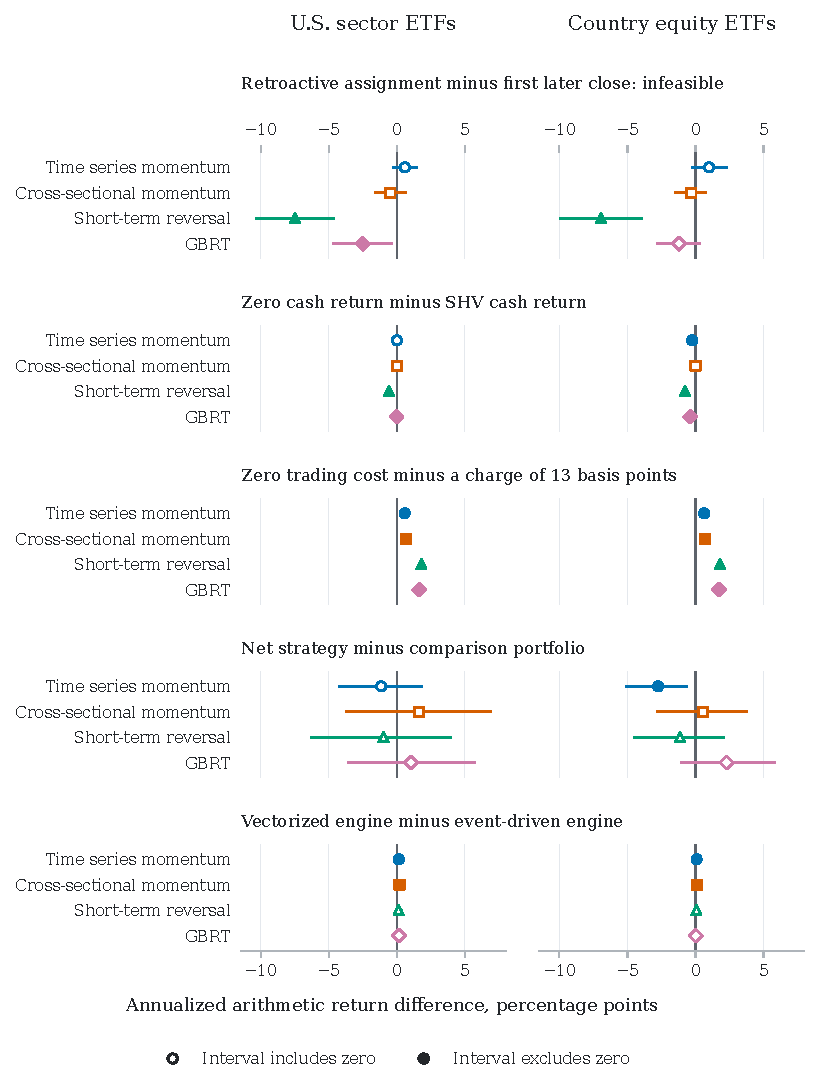
\includegraphics[width=\textwidth]{contract_effects_return.pdf}}}
  \parbox{\textwidth}{\small Figure~\thefigure: Changes in annualized arithmetic return, in percentage points. Group headings give the subtraction order. Lines show unstudentized pointwise 95\% percentile intervals from common resamples of circular blocks of 21 sessions. Fitted models, target weights, and seeds stay fixed. Points for the regression model average differences calculated separately for each of the five seeds. Hollow markers identify intervals including zero, using unrounded bounds. Some intervals are narrower than their markers at this common scale. Retroactive assignment is infeasible and can move the initial entry charge outside the evaluation window. SHV remains the reporting benchmark when cash earns zero.}
\end{center}

\begin{center}
  \centering
  \leavevmode\vbox{\refstepcounter{figure}%
  \label{fig:contract-sharpe}%
  \hbox{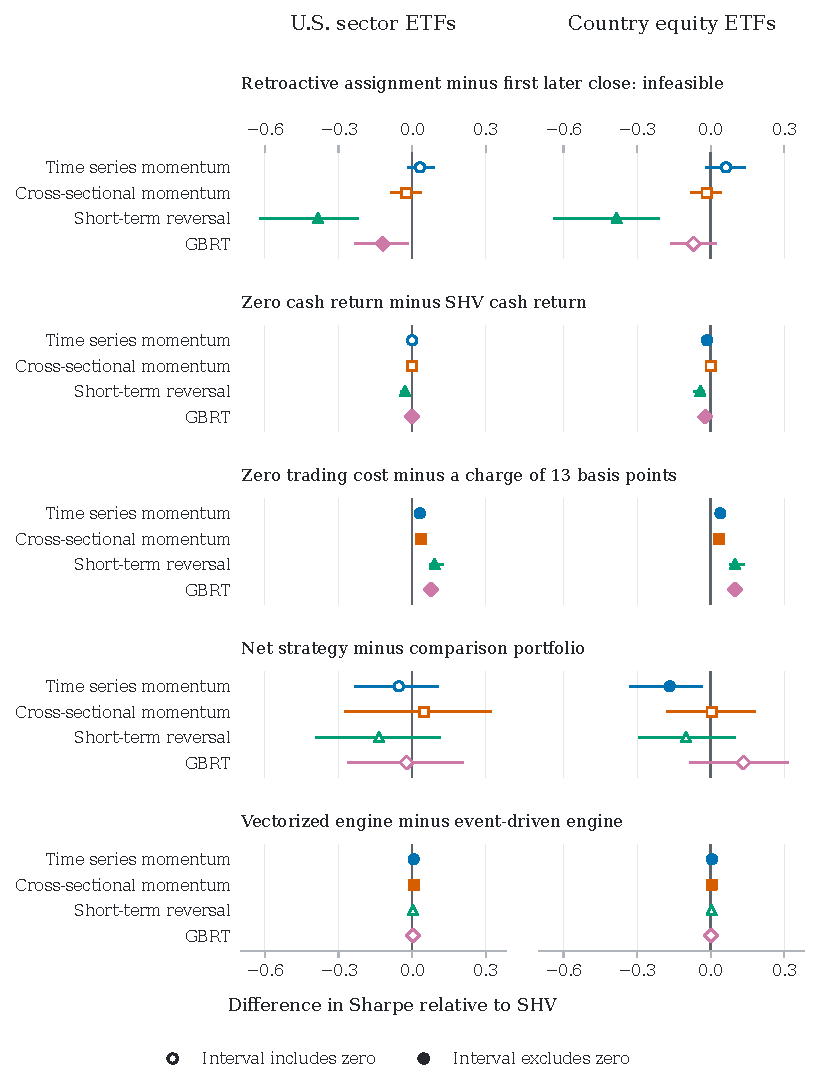
\includegraphics[width=\textwidth]{contract_effects_sharpe.pdf}}}
  \parbox{\textwidth}{\small Figure~\thefigure: Changes in Sharpe relative to SHV under the five signed comparisons. Lines show unstudentized pointwise 95\% percentile intervals from \ExpansionBootstrapReplications{} common draws using circular blocks of 21 sessions. The draws vary aligned dates while retaining the fitted models, target weights, and five seeds. Points for the regression model average the five Sharpe differences calculated separately for each seed. Hollow markers identify intervals including zero, using unrounded bounds; some intervals are narrower than their markers. Retroactive assignment uses an infeasible execution chronology. Zero cash credit changes cash income while SHV remains the Sharpe benchmark.}
\end{center}

\begin{center}
  \centering
  \leavevmode\vbox{\refstepcounter{figure}%
  \label{fig:seed-sensitivity}%
  \hbox{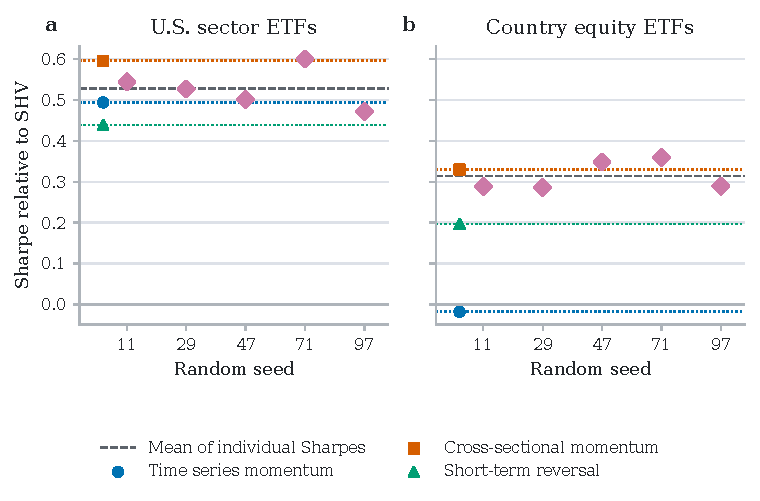
\includegraphics[width=0.90\textwidth]{learned_seed_sensitivity.pdf}}}
  \parbox{0.90\textwidth}{\small Figure~\thefigure: Baseline Sharpe relative to SHV for five model seeds in each ETF set. Diamonds show the regression model's Sharpe for each seed; dashed lines show the mean of the five Sharpes. Dotted lines and their leftmost markers show where each rule's Sharpe falls relative to the seed values. The spread describes these runs on shared history. Inference over a population of seeds requires a separate sampling design.}
\end{center}

\begin{center}
  \centering
  \leavevmode\vbox{\refstepcounter{figure}%
  \label{fig:engine-sensitivity}%
  \hbox{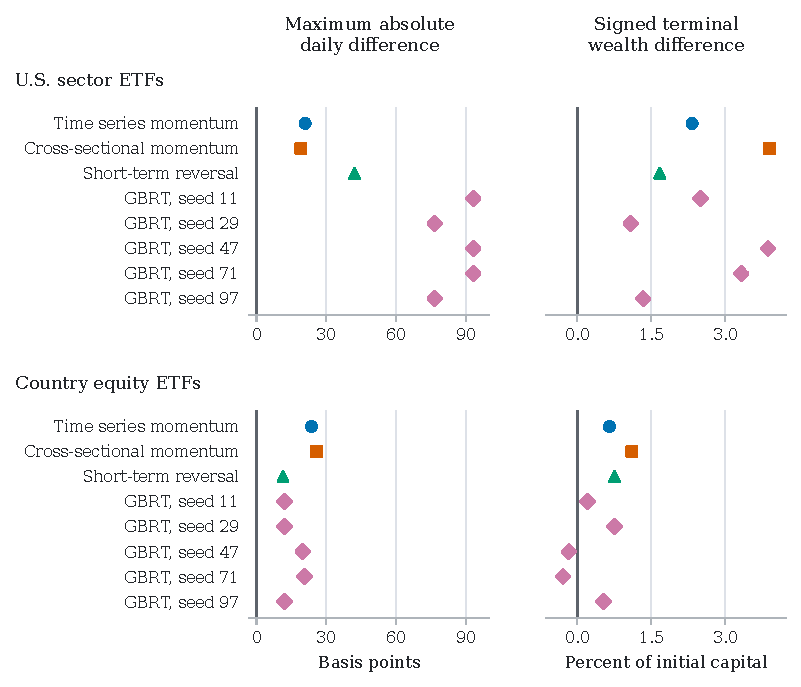
\includegraphics[width=\textwidth]{engine_conformance.pdf}}}
  \parbox{\textwidth}{\small Figure~\thefigure: Engine differences for each rule and each seed of the regression model. Daily maxima measure the largest absolute return difference, in basis points. Terminal gaps subtract event engine wealth from vectorized wealth, as a percentage of initial capital. A large daily discrepancy can coexist with a small terminal gap as differences accumulate with opposing signs. The event engine holds accounting quantities fixed between trades; the vectorized convention resets weights daily. Trade accounting and sizing after costs also differ.}
\end{center}

\section{Retrospective block length sensitivity}

\begin{center}
  \centering
  \leavevmode\vbox{\refstepcounter{figure}%
  \label{fig:block-sensitivity}%
  \hbox{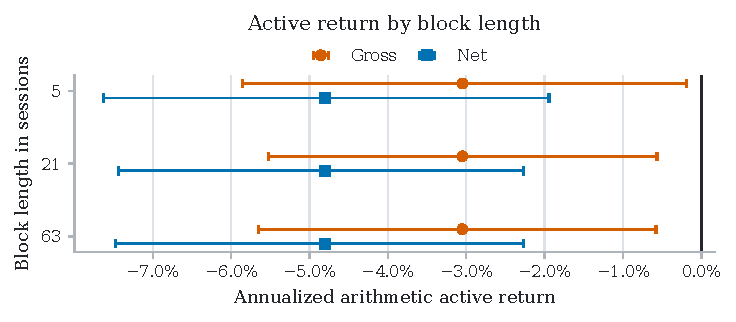
\includegraphics[width=0.88\textwidth]{bootstrap_robustness.pdf}}}
  \parbox{0.88\textwidth}{\small Figure~\thefigure: Annualized arithmetic active return relative to the basket at actual exposure before costs. Intervals are pointwise 95\% bootstrap percentiles for circular blocks of 5, 21, and 63 sessions. Gross subtracts the basket return before costs from the strategy return before costs. Net deducts trading costs from the strategy return and uses the same basket return before costs.}
\end{center}

\section{Retrospective engine comparison}

\begin{center}
  \centering
  \leavevmode\vbox{\refstepcounter{figure}%
  \label{fig:engine-comparison}%
  \hbox{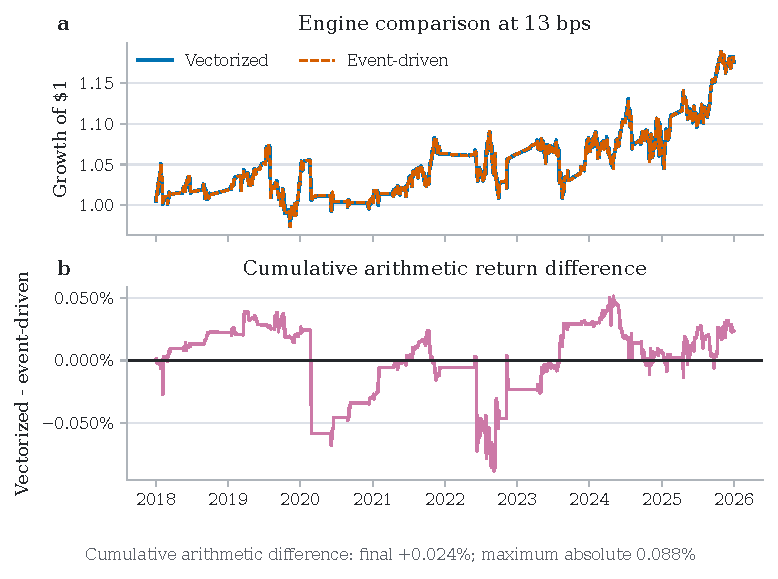
\includegraphics[width=0.92\textwidth]{engine_comparison.pdf}}}
  \parbox{0.92\textwidth}{\small Figure~\thefigure: Subplot a shows growth of one dollar under the two engines. Subplot b shows the arithmetic sum of daily return differences, subtracting event engine returns from vectorized engine returns. This sum differs from subtracting the compounded wealth paths in subplot a. The event engine holds accounting quantities valued at adjusted closing prices fixed between rebalances and allows portfolio weights to drift.}
\end{center}

\clearpage
\section{Retrospective cost and overlay sensitivity}

\begin{center}
  \centering
  \leavevmode\vbox{\refstepcounter{figure}%
  \label{fig:sensitivity}%
  \hbox{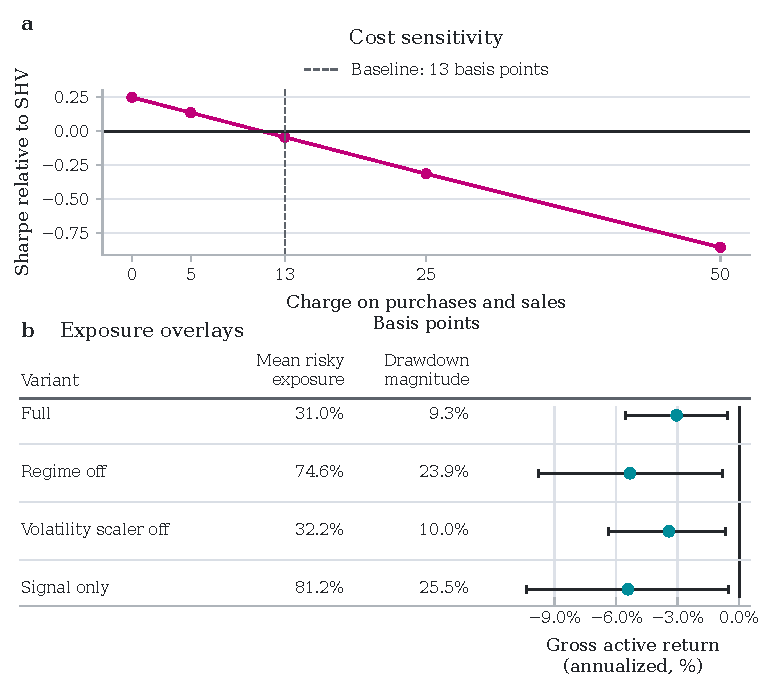
\includegraphics[width=0.92\textwidth]{sensitivity_and_ablation.pdf}}}
  \parbox{0.92\textwidth}{\small Figure~\thefigure: Retrospective sensitivity to trading costs and exposure overlays. Subplot a gives Sharpe relative to SHV under proportional charges on purchases and sales. Subplot b gives gross annualized arithmetic active return relative to the basket at each variant's actual exposure before costs, with pointwise 95\% intervals from common draws using circular blocks of 21 sessions. The columns give mean risky exposure and maximum net drawdown magnitude. Each interval describes a variant's level relative to its own basket; an interval for an overlay effect would require a difference between variants.}
\end{center}

The overlays change how much capital is exposed to risky assets. Removing the regime rule raises mean risky exposure and deepens the maximum drawdown; removing both overlays makes these changes larger. All four intervals for gross active return lie below zero relative to the basket at each variant's actual exposure. The comparisons retain the retrospective generator defect and measure the joint consequences of changes in exposure and the return path.

Positive compound growth can coexist with a shortfall against cash. In the cost grid, Sharpe relative to SHV falls from 0.14 at 5 basis points per dollar bought or sold to $-0.04$ at 13 basis points. CAGR remains positive at 0.40\% under a charge of 25 basis points and falls to $-2.93\%$ at 50 basis points. Complete accounting reruns on the same target weights measure sensitivity to the five assumed charges, with SHV retained as the Sharpe benchmark.

\clearpage
\section{Expansion target specification}
\label{app:expansion-targets}

Time series momentum keeps every asset with a positive simple return over 252 sessions and assigns equal weight among those assets. If none qualify, the target is cash. Cross-sectional momentum ranks simple returns from session $t-252$ to session $t-21$, breaks ties by ascending symbol, and assigns one-third to each of the three assets with the highest returns. The rule fills all three slots even when a selected return is negative.

Short-term reversal ranks simple returns over 5 sessions and keeps up to three assets with the lowest strictly negative returns. Each receives one-third of capital. Any unused slot remains in cash, so a single qualifying asset receives the same weight as one member of a selection of three assets.

A single gradient boosting specification produces the regression model's target weights through the same allocation record interface as the three rules. Each record contains the decision time, symbol, and target weight.

For each decision, we calculate and store features from prices available at that close. The features comprise log returns over 5, 21, 63, 126, and 252 sessions, the sample standard deviation of daily log returns over 21 and 63 sessions, the price divided by its high over the trailing 252 sessions minus one, and ordinal cross-sectional ranks of log returns over 21 and 252 sessions. The ranks use the scale $[0,1]$. The model uses these features without symbol indicators, standardization, or winsorization. The label is the log return over the following 21 sessions. It starts at the decision close, one close before portfolio entry, so the forecast window differs from the executable holding period.

At each monthly decision, we fit a separate model for each seed to asset observations pooled within the ETF set. Training includes only rows whose label endpoint falls on or before that close. It keeps up to the latest 60 decision months with mature labels and requires at least 24. Each fit uses 100 trees of depth 2, learning rate 0.03, minimum leaf size 10, subsample 0.8, and squared error loss, under a limit of one thread. The seeds are 11, 29, 47, 71, and 97.

After fitting, the generator keeps up to three assets with the highest strictly positive predictions, breaks ties by ascending symbol, and assigns one-third to each. The remainder stays in cash. A perturbation test changes prices after a cutoff and checks that this generator's target at the cutoff stays unchanged. Each additional generator needs its own checks on information availability.

\clearpage
\section{Historical variation within the expansion study}
\label{app:expansion-followups}

These descriptive analyses were added during revision after inspection of the aggregate results. They retain the original ETF sets, target weights, model settings, and accounting rules. Outcomes for each calendar year and the fitting paths for the five fixed seeds describe temporal variation and variation among model runs, respectively \citep{bouthillier2021variance}.

\subsection{Performance by calendar year}

For each baseline run and year $y$, we calculate
\begin{equation}
  A_y = \frac{252}{n_y}\sum_{t\in y}
  \left(r_t^{\mathrm{net}}-r_t^{\mathrm{SHV}}\right),
  \label{eq:annual-excess}
\end{equation}
where $n_y$ counts the observed sessions in that year. The slices retain the
holdings, returns across year boundaries, and costs from the continuous evaluation.
Weighting the annual values by their session counts recovers the full sample
annualized arithmetic excess return, $\sum_y n_y A_y / \sum_y n_y$. Figure~\ref{fig:yearly-performance} shows every calendar year
in the evaluation window. Entries for the regression model average the five individual seed values.

The ordering over the full sample combines different annual outcomes on the same history. All four country strategies have negative annualized excess returns over SHV in 2018 and 2022, and positive values in 2019, 2021, 2023, and 2025. The sector strategies diverge in 2022: cross-sectional momentum and reversal earn positive arithmetic returns above SHV, while the mean for the regression model is negative. Gradient boosting leads the sector set in 2021 and 2024; cross-sectional momentum leads in 2020, 2022, and 2025.

\begin{center}
  \leavevmode\vbox{\refstepcounter{figure}%
  \label{fig:yearly-performance}%
  \hbox{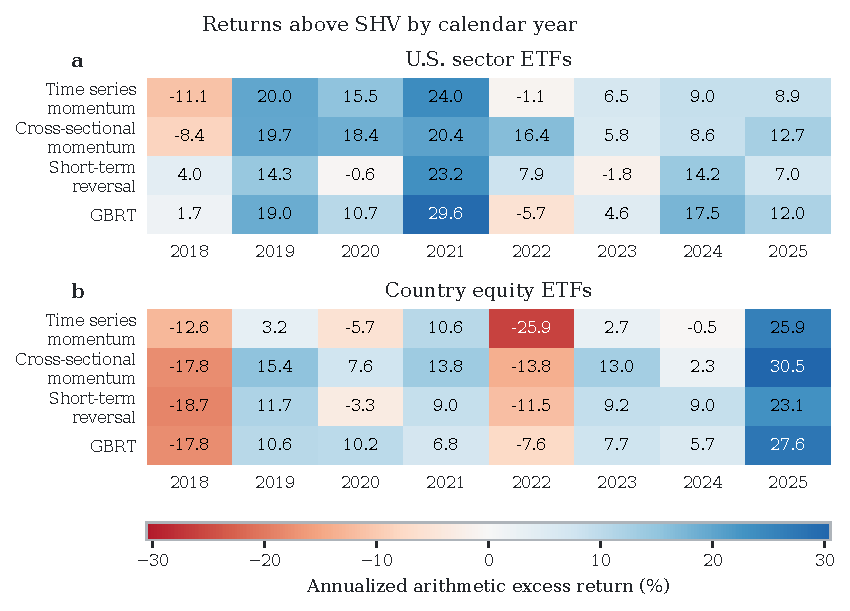
\includegraphics[width=\textwidth]{yearly_performance.pdf}}}
  \parbox{\textwidth}{\small Figure~\thefigure: Baseline performance by calendar year as defined in Equation~\ref{eq:annual-excess}, expressed in percent per year. Each cell uses the original continuous portfolio path after costs and subtracts the aligned daily SHV return. Cells for the regression model average five individual seed values. Both subplots use the same color scale centered at zero. The annual slices describe temporal variation within the historical evaluation sample.}
\end{center}

\clearpage
\subsection{Accounting effects by seed}

Figure~\ref{fig:seed-contract-effects} separates the five fixed seeds in each accounting comparison. Each cell subtracts two Sharpes for the same seed and ETF set, following the five defined subtraction orders. Averaging a column recovers the regression model's point estimate in Figure~\ref{fig:contract-sharpe}. The common color scale compares magnitudes; numerical labels preserve small cash and engine differences.

The seed mean can conceal differences in direction. Against the comparison portfolio after trading costs, the sector regression model has a negative Sharpe difference for every seed except 71; every country seed has a positive difference. Country engine differences change sign across seeds despite a positive mean. By contrast, cash, cost, and retroactive timing effects each have a consistent sign across all ten paths for the regression model.

Each row follows monthly fits that reuse the same integer seed. The five rows share market observations and one training specification; their spread describes the portfolio paths generated by those fits. The intervals in Figure~\ref{fig:contract-sharpe} measure a different source of variation: they resample dates while retaining all five paths.

\begin{center}
  \leavevmode\vbox{\refstepcounter{figure}%
  \label{fig:seed-contract-effects}%
  \hbox{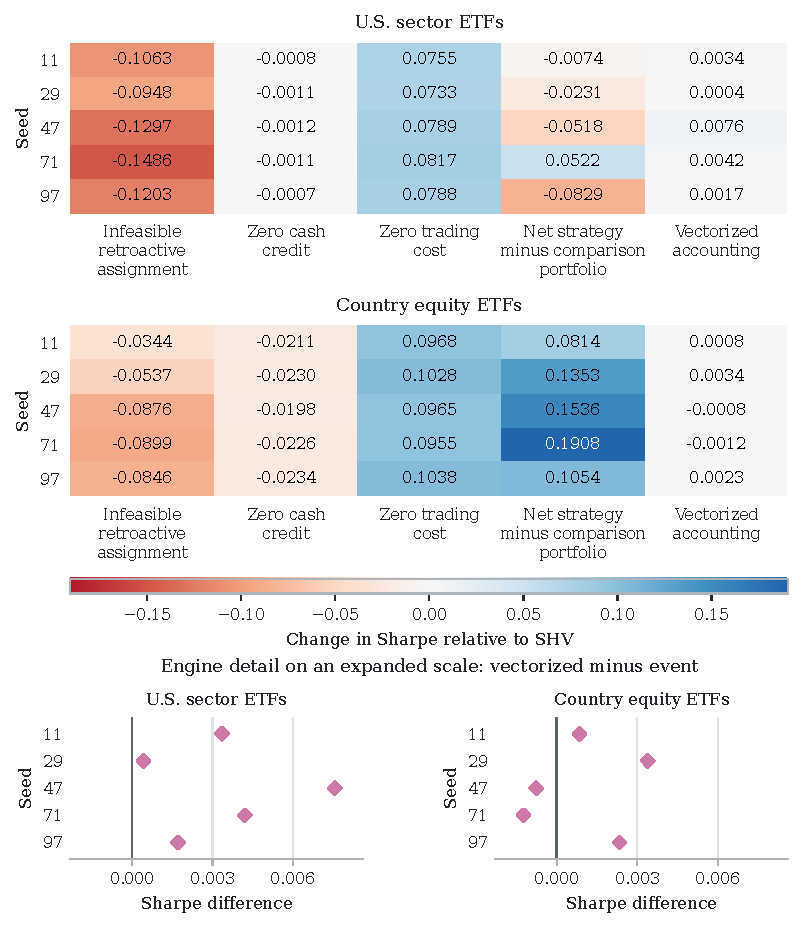
\includegraphics[width=\textwidth]{seed_contract_effects.pdf}}}
  \parbox{\textwidth}{\small Figure~\thefigure: Changes in Sharpe relative to SHV within each of the five seeds for the regression model. Each matrix column subtracts baseline Sharpe from the displayed convention's Sharpe, except the comparison portfolio column, which reports strategy minus comparison portfolio, both after trading costs. The comparison portfolio matches that seed's target exposure. Retroactive assignment is infeasible and may also move the initial entry charge outside the evaluation window. Matrix colors share a scale centered at zero. The engine detail uses a separate horizontal scale, common to both ETF sets, to show the small positive and negative differences. All marks are point estimates.}
\end{center}

\clearpage
\subsection{Exposure and trading}

Table~\ref{tab:expansion-trading} distinguishes risky exposure, trading activity, and the return deducted for costs along each baseline path. Gross traded notional sums purchases and sales relative to portfolio value immediately before each trade, counting both sides of a rotation and changes in total risky exposure. The cost column is $252\,\operatorname{mean}(d_t)$, where $d_t=r_t^{\mathrm{gross}}-r_t^{\mathrm{net}}$ is the event engine's cost deduction. Both returns use the previous close's portfolio value as their denominator. This arithmetic deduction measures costs incurred along the observed path; a separate rerun with zero modeled cost also changes subsequent wealth and trade sizes. The distinction depends on when holdings, trades, and costs enter portfolio valuation \citep{boyd2017trading}.

\refstepcounter{table}
\label{tab:expansion-trading}
\begin{center}
  \parbox{\textwidth}{\small Table~\thetable: Baseline mean risky exposure, annual gross traded notional as a multiple of portfolio value, and annualized arithmetic cost deduction. Entries for the regression model average five individual metrics. All paths use the same charge of 13 basis points on purchases and sales.}
  \smallskip
  \setlength{\tabcolsep}{4.5pt}
  \begin{tabular}{@{}llrrr@{}}
    \toprule
    Fund set & Strategy & \shortstack{Mean risky\\exposure} & \shortstack{Annual gross\\traded notional} & \shortstack{Annualized\\cost deduction} \\
    \midrule
    \ExpansionTradingRows
    \bottomrule
  \end{tabular}
\end{center}

The mean annual gross traded notional for gradient boosting is more than twice that of cross-sectional momentum in both ETF sets. At the same flat trading charge, gradient boosting incurs larger cost deductions. For country ETFs, it also has lower mean risky exposure. These return and Sharpe comparisons combine differences in exposure, allocation, and trading over the full historical window. Estimating capacity or market impact would require trading size, liquidity, and execution data.

\par\medskip\noindent
\begin{minipage}{\textwidth}
\section{Evidence summary}
\label{app:evidence}

\begin{center}
\begin{tabular}{>{\raggedright\arraybackslash}p{0.20\linewidth}
                >{\raggedright\arraybackslash}p{0.34\linewidth}
                >{\raggedright\arraybackslash}p{0.36\linewidth}}
  \toprule
  Evidence & Observed property & Further evidence needed \\
  \midrule
  Exact daily decomposition & Net excess over cash equals four arithmetic components, daily and within each joint resample. & A causal design, a geometric linking rule, or implementable portfolios for those respective interpretations. \\
  Checks on allocation records & Records have valid decision times, complete symbol coverage, and admissible target weights. & Generator information checks, execution alignment, cash observations, and tests of future target generation. \\
  Comparison under common targets & The accounting convention changes while the allocation records stay fixed. & Broader cases for a general direction of bias, generator checks for information timing, and new targets for a different strategy. \\
  Conditional comparison portfolio & The basket after trading costs shares the strategy's target exposure path. & A separately defined benchmark for an independent comparison, or a causal design for attribution of skill. \\
  Comparison of two engines & Two stated accounting conventions produce a measurable return difference. & External accounting oracles for correctness and a wider implementation sample for typical error. \\
  Simulated state failures & Simulated order tests reject stale writes, uncertain retries, and unresolved replacements for the same symbol. & Account exposure checks, delivery tests with concurrent clients, authenticated transport, venue trials, and deployment controls. \\
  \bottomrule
\end{tabular}
\end{center}
\end{minipage}

\ifquantcortexreview
  \clearpage
  \section*{NeurIPS Paper Checklist}

\begin{enumerate}

\item {\bf Claims}
    \item[] Question: Do the main claims made in the abstract and introduction accurately reflect the paper's contributions and scope?
    \item[] Answer: \answerYes{}
    \item[] Justification: The abstract and Section 1 describe an audit of historical portfolio performance under explicit trading and accounting rules. The results in Section 5 support comparisons within the histories and strategy specifications studied, subject to the limits in Section~\ref{sec:limitations}.
    \item[] Guidelines:
    \begin{itemize}
        \item The answer \answerNA{} means that the abstract and introduction do not include the claims made in the paper.
        \item The abstract and/or introduction should clearly state the claims made, including the contributions made in the paper and important assumptions and limitations. A \answerNo{} or \answerNA{} answer to this question will not be perceived well by the reviewers. 
        \item The claims made should match theoretical and experimental results, and reflect how much the results can be expected to generalize to other settings. 
        \item It is fine to include aspirational goals as motivation as long as it is clear that these goals are not attained by the paper. 
    \end{itemize}

\item {\bf Limitations}
    \item[] Question: Does the paper discuss the limitations of the work performed by the authors?
    \item[] Answer: \answerYes{}
    \item[] Justification: Section~\ref{sec:limitations} discusses historical reuse, incomplete trial records, dependence among the cases, and the conditional scope of the intervals. Appendices~\ref{app:scope} and~\ref{app:reproducibility} explain the limits of the accounting assumptions, ETF selection, cash and cost proxies, data access, and simulated execution tests.
    \item[] Guidelines:
    \begin{itemize}
        \item The answer \answerNA{} means that the paper has no limitation while the answer \answerNo{} means that the paper has limitations, but those are not discussed in the paper. 
        \item The authors are encouraged to create a separate ``Limitations'' section in their paper.
        \item The paper should point out any strong assumptions and how robust the results are to violations of these assumptions (e.g., independence assumptions, noiseless settings, model well-specification, asymptotic approximations only holding locally). The authors should reflect on how these assumptions might be violated in practice and what the implications would be.
        \item The authors should reflect on the scope of the claims made, e.g., if the approach was only tested on a few datasets or with a few runs. In general, empirical results often depend on implicit assumptions, which should be articulated.
        \item The authors should reflect on the factors that influence the performance of the approach. For example, a facial recognition algorithm may perform poorly when image resolution is low or images are taken in low lighting. Or a speech-to-text system might not be used reliably to provide closed captions for online lectures because it fails to handle technical jargon.
        \item The authors should discuss the computational efficiency of the proposed algorithms and how they scale with dataset size.
        \item If applicable, the authors should discuss possible limitations of their approach to address problems of privacy and fairness.
        \item While the authors might fear that complete honesty about limitations might be used by reviewers as grounds for rejection, a worse outcome might be that reviewers discover limitations that aren't acknowledged in the paper. The authors should use their best judgment and recognize that individual actions in favor of transparency play an important role in developing norms that preserve the integrity of the community. Reviewers will be specifically instructed to not penalize honesty concerning limitations.
    \end{itemize}

\item {\bf Theory assumptions and proofs}
    \item[] Question: For each theoretical result, does the paper provide the full set of assumptions and a complete (and correct) proof?
    \item[] Answer: \answerNA{}
    \item[] Justification: The contribution is an empirical audit using established estimators, with no new theoretical results. The equations in Section 3 and Appendix~\ref{app:scope} define the accounting and give direct algebraic decompositions.
    \item[] Guidelines:
    \begin{itemize}
        \item The answer \answerNA{} means that the paper does not include theoretical results. 
        \item All the theorems, formulas, and proofs in the paper should be numbered and cross-referenced.
        \item All assumptions should be clearly stated or referenced in the statement of any theorems.
        \item The proofs can either appear in the main paper or the supplemental material, but if they appear in the supplemental material, the authors are encouraged to provide a short proof sketch to provide intuition. 
        \item Inversely, any informal proof provided in the core of the paper should be complemented by formal proofs provided in appendix or supplemental material.
        \item Theorems and Lemmas that the proof relies upon should be properly referenced. 
    \end{itemize}

    \item {\bf Experimental result reproducibility}
    \item[] Question: Does the paper fully disclose all the information needed to reproduce the main experimental results of the paper to the extent that it affects the main claims and/or conclusions of the paper (regardless of whether the code and data are provided or not)?
    \item[] Answer: \answerNo{}
    \item[] Justification: Section 4 and Appendices~\ref{app:retrospective} and~\ref{app:expansion-targets} specify the experiments, but the public materials do not provide a way to recover the exact original price inputs. Appendix~\ref{app:reproducibility} explains why later downloads may differ and which accounting checks can be reproduced with synthetic data.
    \item[] Guidelines:
    \begin{itemize}
        \item The answer \answerNA{} means that the paper does not include experiments.
        \item If the paper includes experiments, a \answerNo{} answer to this question will not be perceived well by the reviewers: Making the paper reproducible is important, regardless of whether the code and data are provided or not.
        \item If the contribution is a dataset and\slash or model, the authors should describe the steps taken to make their results reproducible or verifiable. 
        \item Depending on the contribution, reproducibility can be accomplished in various ways. For example, if the contribution is a novel architecture, describing the architecture fully might suffice, or if the contribution is a specific model and empirical evaluation, it may be necessary to either make it possible for others to replicate the model with the same dataset, or provide access to the model. In general. releasing code and data is often one good way to accomplish this, but reproducibility can also be provided via detailed instructions for how to replicate the results, access to a hosted model (e.g., in the case of a large language model), releasing of a model checkpoint, or other means that are appropriate to the research performed.
        \item While NeurIPS does not require releasing code, the conference does require all submissions to provide some reasonable avenue for reproducibility, which may depend on the nature of the contribution. For example
        \begin{enumerate}
            \item If the contribution is primarily a new algorithm, the paper should make it clear how to reproduce that algorithm.
            \item If the contribution is primarily a new model architecture, the paper should describe the architecture clearly and fully.
            \item If the contribution is a new model (e.g., a large language model), then there should either be a way to access this model for reproducing the results or a way to reproduce the model (e.g., with an open-source dataset or instructions for how to construct the dataset).
            \item We recognize that reproducibility may be tricky in some cases, in which case authors are welcome to describe the particular way they provide for reproducibility. In the case of closed-source models, it may be that access to the model is limited in some way (e.g., to registered users), but it should be possible for other researchers to have some path to reproducing or verifying the results.
        \end{enumerate}
    \end{itemize}


\item {\bf Open access to data and code}
    \item[] Question: Does the paper provide open access to the data and code, with sufficient instructions to faithfully reproduce the main experimental results, as described in supplemental material?
    \item[] Answer: \answerNo{}
    \item[] Justification: The code, aggregate results, environment specification, and synthetic examples are public. The original price matrices and empirical target weights are not distributed, as described in Appendix~\ref{app:reproducibility}.
    \item[] Guidelines:
    \begin{itemize}
        \item The answer \answerNA{} means that paper does not include experiments requiring code.
        \item Please see the NeurIPS code and data submission guidelines (\url{https://neurips.cc/public/guides/CodeSubmissionPolicy}) for more details.
        \item While we encourage the release of code and data, we understand that this might not be possible, so \answerNo{} is an acceptable answer. Papers cannot be rejected simply for not including code, unless this is central to the contribution (e.g., for a new open-source benchmark).
        \item The instructions should contain the exact command and environment needed to run to reproduce the results. See the NeurIPS code and data submission guidelines (\url{https://neurips.cc/public/guides/CodeSubmissionPolicy}) for more details.
        \item The authors should provide instructions on data access and preparation, including how to access the raw data, preprocessed data, intermediate data, and generated data, etc.
        \item The authors should provide scripts to reproduce all experimental results for the new proposed method and baselines. If only a subset of experiments are reproducible, they should state which ones are omitted from the script and why.
        \item At submission time, to preserve anonymity, the authors should release anonymized versions (if applicable).
        \item Providing as much information as possible in supplemental material (appended to the paper) is recommended, but including URLs to data and code is permitted.
    \end{itemize}


\item {\bf Experimental setting/details}
    \item[] Question: Does the paper specify all the training and test details (e.g., data splits, hyperparameters, how they were chosen, type of optimizer) necessary to understand the results?
    \item[] Answer: \answerYes{}
    \item[] Justification: Section 4 specifies the data periods, ETF sets, trading rules, accounting conventions, and comparison design. Appendices~\ref{app:retrospective} and~\ref{app:expansion-targets} give the strategy settings and the regression model's features, label, training window, hyperparameters, and seeds; Section~\ref{sec:limitations} explains historical reuse and the incomplete record of earlier trials.
    \item[] Guidelines:
    \begin{itemize}
        \item The answer \answerNA{} means that the paper does not include experiments.
        \item The experimental setting should be presented in the core of the paper to a level of detail that is necessary to appreciate the results and make sense of them.
        \item The full details can be provided either with the code, in appendix, or as supplemental material.
    \end{itemize}

\newpage
\item {\bf Experiment statistical significance}
    \item[] Question: Does the paper report error bars suitably and correctly defined or other appropriate information about the statistical significance of the experiments?
    \item[] Answer: \answerYes{}
    \item[] Justification: Sections 3 to 5 define pointwise 95\% percentile intervals from circular block resampling, using common sampled dates for each comparison and sensitivity checks on block length. Section~\ref{sec:limitations} and Appendix~\ref{app:scope} describe the conditioning assumptions and limits concerning temporal dependence, model selection, seed variation, and multiple comparisons.
    \item[] Guidelines:
    \begin{itemize}
        \item The answer \answerNA{} means that the paper does not include experiments.
        \item The authors should answer \answerYes{} if the results are accompanied by error bars, confidence intervals, or statistical significance tests, at least for the experiments that support the main claims of the paper.
        \item The factors of variability that the error bars are capturing should be clearly stated (for example, train/test split, initialization, random drawing of some parameter, or overall run with given experimental conditions).
        \item The method for calculating the error bars should be explained (closed form formula, call to a library function, bootstrap, etc.)
        \item The assumptions made should be given (e.g., Normally distributed errors).
        \item It should be clear whether the error bar is the standard deviation or the standard error of the mean.
        \item It is OK to report 1-sigma error bars, but one should state it. The authors should preferably report a 2-sigma error bar than state that they have a 96\% CI, if the hypothesis of Normality of errors is not verified.
        \item For asymmetric distributions, the authors should be careful not to show in tables or figures symmetric error bars that would yield results that are out of range (e.g., negative error rates).
        \item If error bars are reported in tables or plots, the authors should explain in the text how they were calculated and reference the corresponding figures or tables in the text.
    \end{itemize}

\item {\bf Experiments compute resources}
    \item[] Question: For each experiment, does the paper provide sufficient information on the computer resources (type of compute workers, memory, time of execution) needed to reproduce the experiments?
    \item[] Answer: \answerNo{}
    \item[] Justification: The accompanying documentation gives hardware details and aggregate timings for an earlier version of the experiments. It does not supply runtimes for each current experiment, peak memory use, or total research compute, including development runs.
    \item[] Guidelines:
    \begin{itemize}
        \item The answer \answerNA{} means that the paper does not include experiments.
        \item The paper should indicate the type of compute workers CPU or GPU, internal cluster, or cloud provider, including relevant memory and storage.
        \item The paper should provide the amount of compute required for each of the individual experimental runs as well as estimate the total compute. 
        \item The paper should disclose whether the full research project required more compute than the experiments reported in the paper (e.g., preliminary or failed experiments that didn't make it into the paper). 
    \end{itemize}
    
\newpage
\item {\bf Code of ethics}
    \item[] Question: Does the research conducted in the paper conform, in every respect, with the NeurIPS Code of Ethics \url{https://neurips.cc/public/EthicsGuidelines}?
    \item[] Answer: \answerNo{}
    \item[] Justification: Provider permission to publish derived aggregates remains unverified, as explained in Appendix~\ref{app:reproducibility}. We therefore cannot affirm full compliance with the data use terms.
    \item[] Guidelines:
    \begin{itemize}
        \item The answer \answerNA{} means that the authors have not reviewed the NeurIPS Code of Ethics.
        \item If the authors answer \answerNo, they should explain the special circumstances that require a deviation from the Code of Ethics.
        \item The authors should make sure to preserve anonymity (e.g., if there is a special consideration due to laws or regulations in their jurisdiction).
    \end{itemize}


\item {\bf Broader impacts}
    \item[] Question: Does the paper discuss both potential positive societal impacts and negative societal impacts of the work performed?
    \item[] Answer: \answerYes{}
    \item[] Justification: Section~\ref{sec:limitations} describes how inspecting performance assumptions can inform investment decisions, and how treating conditional historical comparisons as grounds for live deployment could expose investors to losses. Appendix~\ref{app:scope} explains the additional market and operational evidence needed to assess live use.
    \item[] Guidelines:
    \begin{itemize}
        \item The answer \answerNA{} means that there is no societal impact of the work performed.
        \item If the authors answer \answerNA{} or \answerNo, they should explain why their work has no societal impact or why the paper does not address societal impact.
        \item Examples of negative societal impacts include potential malicious or unintended uses (e.g., disinformation, generating fake profiles, surveillance), fairness considerations (e.g., deployment of technologies that could make decisions that unfairly impact specific groups), privacy considerations, and security considerations.
        \item The conference expects that many papers will be foundational research and not tied to particular applications, let alone deployments. However, if there is a direct path to any negative applications, the authors should point it out. For example, it is legitimate to point out that an improvement in the quality of generative models could be used to generate Deepfakes for disinformation. On the other hand, it is not needed to point out that a generic algorithm for optimizing neural networks could enable people to train models that generate Deepfakes faster.
        \item The authors should consider possible harms that could arise when the technology is being used as intended and functioning correctly, harms that could arise when the technology is being used as intended but gives incorrect results, and harms following from (intentional or unintentional) misuse of the technology.
        \item If there are negative societal impacts, the authors could also discuss possible mitigation strategies (e.g., gated release of models, providing defenses in addition to attacks, mechanisms for monitoring misuse, mechanisms to monitor how a system learns from feedback over time, improving the efficiency and accessibility of ML).
    \end{itemize}
    
\newpage
\item {\bf Safeguards}
    \item[] Question: Does the paper describe safeguards that have been put in place for responsible release of data or models that have a high risk for misuse (e.g., pre-trained language models, image generators, or scraped datasets)?
    \item[] Answer: \answerNA{}
    \item[] Justification: The released evaluation code, synthetic examples, and aggregate financial results do not include a model or dataset with the high misuse risk addressed by this question. The risks of relying on simulated performance for investment decisions are discussed in Section~\ref{sec:limitations}.
    \item[] Guidelines:
    \begin{itemize}
        \item The answer \answerNA{} means that the paper poses no such risks.
        \item Released models that have a high risk for misuse or dual-use should be released with necessary safeguards to allow for controlled use of the model, for example by requiring that users adhere to usage guidelines or restrictions to access the model or implementing safety filters. 
        \item Datasets that have been scraped from the Internet could pose safety risks. The authors should describe how they avoided releasing unsafe images.
        \item We recognize that providing effective safeguards is challenging, and many papers do not require this, but we encourage authors to take this into account and make a best faith effort.
    \end{itemize}

\item {\bf Licenses for existing assets}
    \item[] Question: Are the creators or original owners of assets (e.g., code, data, models), used in the paper, properly credited and are the license and terms of use explicitly mentioned and properly respected?
    \item[] Answer: \answerNo{}
    \item[] Justification: The acknowledgments credit Yahoo Finance, yfinance, and the scientific software contributors. As Appendix~\ref{app:reproducibility} explains, permission to publish derived results or redistribute the source data remains unverified, and the price matrices are not distributed.
    \item[] Guidelines:
    \begin{itemize}
        \item The answer \answerNA{} means that the paper does not use existing assets.
        \item The authors should cite the original paper that produced the code package or dataset.
        \item The authors should state which version of the asset is used and, if possible, include a URL.
        \item The name of the license (e.g., CC-BY 4.0) should be included for each asset.
        \item For scraped data from a particular source (e.g., website), the copyright and terms of service of that source should be provided.
        \item If assets are released, the license, copyright information, and terms of use in the package should be provided. For popular datasets, \href{https://paperswithcode.com/datasets}{\nolinkurl{paperswithcode.com/datasets}} has curated licenses for some datasets. Their licensing guide can help determine the license of a dataset.
        \item For existing datasets that are re-packaged, both the original license and the license of the derived asset (if it has changed) should be provided.
        \item If this information is not available online, the authors are encouraged to reach out to the asset's creators.
    \end{itemize}

\newpage
\item {\bf New assets}
    \item[] Question: Are new assets introduced in the paper well documented and is the documentation provided alongside the assets?
    \item[] Answer: \answerYes{}
    \item[] Justification: Appendix~\ref{app:reproducibility} identifies the available code, environment specification, aggregate results, and synthetic examples. The accompanying documentation describes their use, data formats, experiment settings, and limitations.
    \item[] Guidelines:
    \begin{itemize}
        \item The answer \answerNA{} means that the paper does not release new assets.
        \item Researchers should communicate the details of the dataset\slash code\slash model as part of their submissions via structured templates. This includes details about training, license, limitations, etc. 
        \item The paper should discuss whether and how consent was obtained from people whose asset is used.
        \item At submission time, remember to anonymize your assets (if applicable). You can either create an anonymized URL or include an anonymized zip file.
    \end{itemize}

\item {\bf Crowdsourcing and research with human subjects}
    \item[] Question: For crowdsourcing experiments and research with human subjects, does the paper include the full text of instructions given to participants and screenshots, if applicable, as well as details about compensation (if any)? 
    \item[] Answer: \answerNA{}
    \item[] Justification: The experiments analyze market prices and synthetic accounting cases, without crowdsourcing or human participants.
    \item[] Guidelines:
    \begin{itemize}
        \item The answer \answerNA{} means that the paper does not involve crowdsourcing nor research with human subjects.
        \item Including this information in the supplemental material is fine, but if the main contribution of the paper involves human subjects, then as much detail as possible should be included in the main paper. 
        \item According to the NeurIPS Code of Ethics, workers involved in data collection, curation, or other labor should be paid at least the minimum wage in the country of the data collector. 
    \end{itemize}

\newpage
\item {\bf Institutional review board (IRB) approvals or equivalent for research with human subjects}
    \item[] Question: Does the paper describe potential risks incurred by study participants, whether such risks were disclosed to the subjects, and whether Institutional Review Board (IRB) approvals (or an equivalent approval/review based on the requirements of your country or institution) were obtained?
    \item[] Answer: \answerNA{}
    \item[] Justification: Review for research with human subjects does not apply to this study of market prices and synthetic data, which involves no human participants or personal data.
    \item[] Guidelines:
    \begin{itemize}
        \item The answer \answerNA{} means that the paper does not involve crowdsourcing nor research with human subjects.
        \item Depending on the country in which research is conducted, IRB approval (or equivalent) may be required for any human subjects research. If you obtained IRB approval, you should clearly state this in the paper. 
        \item We recognize that the procedures for this may vary significantly between institutions and locations, and we expect authors to adhere to the NeurIPS Code of Ethics and the guidelines for their institution. 
        \item For initial submissions, do not include any information that would break anonymity (if applicable), such as the institution conducting the review.
    \end{itemize}

\item {\bf Declaration of LLM usage}
    \item[] Question: Does the paper describe the usage of LLMs if it is an important, original, or non-standard component of the core methods in this research? Note that if the LLM is used only for writing, editing, or formatting purposes and does \emph{not} impact the core methodology, scientific rigor, or originality of the research, declaration is not required.
    %this research? 
    \item[] Answer: \answerNA{}
    \item[] Justification: We chose the research methods and used LLMs for coding assistance, checks, and editing. LLMs are not a component of the portfolio models or evaluation method studied in the paper.
    \item[] Guidelines:
    \begin{itemize}
        \item The answer \answerNA{} means that the core method development in this research does not involve LLMs as any important, original, or non-standard components.
        \item Please refer to our LLM policy in the NeurIPS handbook for what should or should not be described.
    \end{itemize}

\end{enumerate}

\fi

\end{document}
